\documentclass{beamer}
\usepackage{tikz}
\usepackage[all]{xy}
\usepackage{amsmath,amssymb}
\usepackage{hyperref}
\usepackage{graphicx}
\usepackage{algorithmic}
\usepackage{multirow}

\DeclareMathOperator*{\argmin}{arg\,min}
\DeclareMathOperator*{\Lik}{Lik}
\DeclareMathOperator*{\PoissonLoss}{PoissonLoss}
\DeclareMathOperator*{\Peaks}{Peaks}
\DeclareMathOperator*{\Segments}{Segments}
\DeclareMathOperator*{\argmax}{arg\,max}
\DeclareMathOperator*{\maximize}{maximize}
\DeclareMathOperator*{\minimize}{minimize}
\newcommand{\sign}{\operatorname{sign}}
\newcommand{\RR}{\mathbb R}
\newcommand{\ZZ}{\mathbb Z}
\newcommand{\NN}{\mathbb N}
\newcommand{\z}{$z = 2, 4, 3, 5, 1$} 

\newcommand{\algo}[1]{\textcolor{#1}{#1}}
\definecolor{PDPA}{HTML}{66C2A5}
\definecolor{CDPA}{HTML}{FC8D62}
\definecolor{GPDPA}{HTML}{4D4D4D}

% Set transparency of non-highlighted sections in the table of
% contents slide.
\setbeamertemplate{section in toc shaded}[default][100]
\AtBeginSection[]
{
  \setbeamercolor{section in toc}{fg=red} 
  \setbeamercolor{section in toc shaded}{fg=black} 
  \begin{frame}
    \tableofcontents[currentsection]
  \end{frame}
}

\begin{document}

\title{Introduction to machine learning and neural networks}

\author{
  Toby Dylan Hocking\\
  toby.hocking@nau.edu\\
  toby.hocking@r-project.org\\
}

\maketitle

\section{Introduction and applications}

\begin{frame}
  \frametitle{Machine learning intro: image classification example}
  ML is all about learning predictive functions $f(x)\approx y$, where 
  \begin{itemize}
  \item Inputs/features $x$ can be easily computed using traditional
    algorithms, e.g. matrix of pixel intensities in an image.
  \item Outputs/labels $y$ are what we want to predict, easy to get by
    asking a human, but hard to compute using traditional algorithms,
    e.g. image class.
  \item Input $x$ = image of digit, output $y\in\{0,1,\dots,9\}$, \\--
    this is a classification problem with 10 classes.\\
  $f(
\includegraphics[height=1cm]{mnist-0})=0$,
  $f(
\includegraphics[height=1cm]{mnist-1})=1$
\item Traditional/unsupervised algorithm: I give you a pixel intensity matrix
  $x\in\RR^{16\times 16}$, you code a function $f$ that returns one of
  the 10 possible digits. Q: how to do that?
  \end{itemize}
\end{frame}

\begin{frame}
  \frametitle{Supervised machine learning algorithms}

  I give you a training data set with paired inputs/outputs, e.g.

  \begin{center}
    \Huge 0 1 2 3 4 5 6 7 8 9

  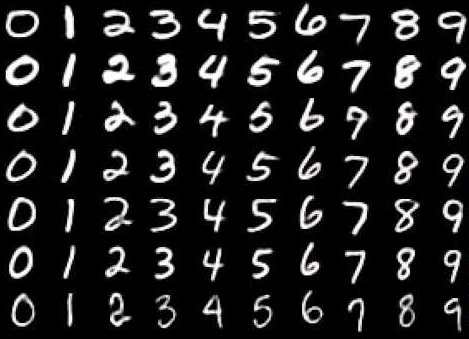
\includegraphics[height=1.9in]{mnist-digits}
  \end{center}

  Your job is to code an algorithm that learns the function $f$ from
  the training data. (you don't code $f$)
  
  \scriptsize Source: github.com/cazala/mnist
\end{frame}


\begin{frame}
  \frametitle{Advantages of supervised machine learning}

  \begin{center}
      \begin{tabular}{cc}
        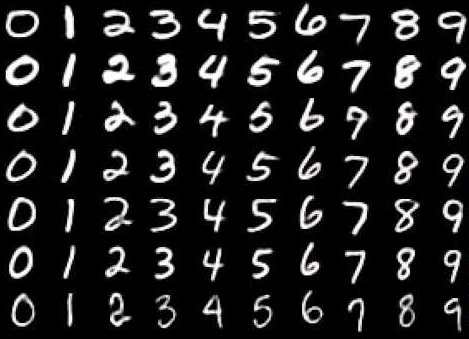
\includegraphics[height=1.5in]{mnist-digits} &
  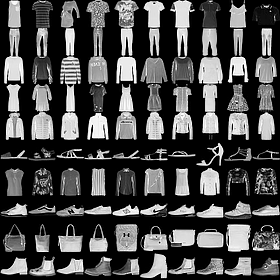
\includegraphics[height=1.5in]{fashion-mnist-sprite-some}  
  \end{tabular}
  \end{center}
  \vskip -0.2cm
  
  \begin{itemize}
  \item Input $x\in\RR^{16\times 16}$, output $y\in\{0,1,\dots,9\}$ types the same!
  \item Can use same learning algorithm regardless of pattern.
  \item Pattern encoded in the labels (not the algorithm).
  \item Useful if there are many un-labeled data, but few labeled data
    (or getting labels is long/costly).
  \item State-of-the-art accuracy (if there is enough training data).
  \end{itemize}

  \scriptsize Sources: github.com/cazala/mnist, github.com/zalandoresearch/fashion-mnist

\end{frame}

\begin{frame}
  \frametitle{Learning two different functions}
  Say \textsc{Learn} is a learning algorithm you have coded.
  \begin{center}
      \begin{tabular}{c}
        \textsc{Learn}(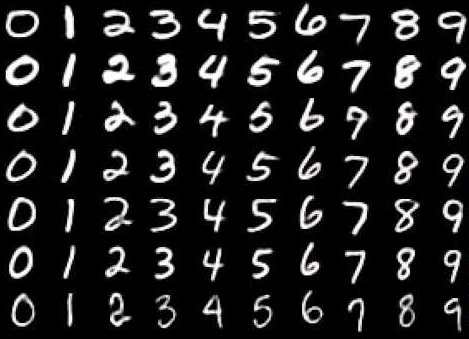
\includegraphics[height=1in]{mnist-digits}) $\rightarrow f$, 
        \textsc{Learn}(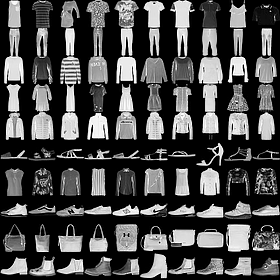
\includegraphics[height=1in]{fashion-mnist-sprite-some}) $\rightarrow g$
  \end{tabular}
  \end{center}
  \begin{itemize}
  \item Then we would expect
    $f(
\includegraphics[height=1cm]{mnist-0})=0$,
    $f(
\includegraphics[height=1cm]{mnist-1})=1$
  \item $g(
\includegraphics[height=1cm]{fashion-mnist-boot})=\text{shoe/0}$,
  $g(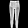
\includegraphics[height=1cm]{fashion-mnist-pants})=\text{pants/1}$
  \item Q: what happens if you do 
    $f(
\includegraphics[height=1cm]{fashion-mnist-boot})$, or
   $g(
\includegraphics[height=1cm]{mnist-0})$?

  \end{itemize}
\end{frame}

\begin{frame}
  \frametitle{Machine learning for cell image classification (CellProfiler)}
  Jones {\it et al.} PNAS 2009. Scoring diverse cellular morphologies in
  image-based screens with iterative feedback and machine learning.

\parbox{2in}{
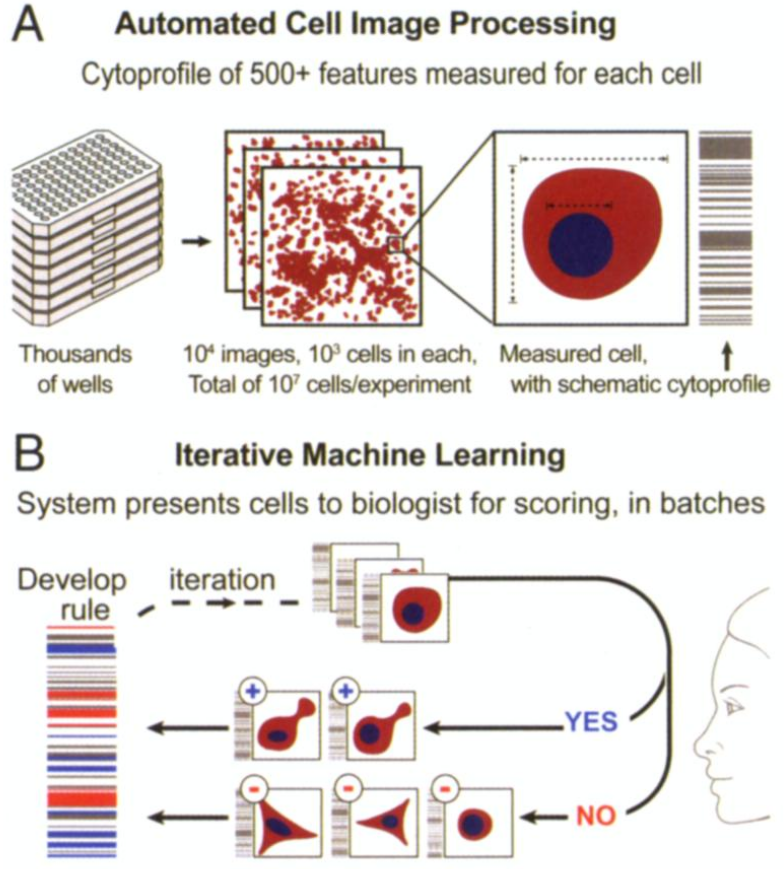
\includegraphics[width=2in]{cellprofiler} 
}
\parbox{2in}{
\begin{itemize}
  \item Input $x$ = image of cell, 
  \item Output $y\in\{\text{yes}, \text{no}\}$ (binary classification),
  \item $f(
\includegraphics[height=1cm]{cellprofiler-yes})=\text{yes}$,
  \item $f(
\includegraphics[height=1cm]{cellprofiler-no})=\text{no}$.
  \end{itemize}
}
\end{frame}

\begin{frame}
  \frametitle{Machine learning for image segmentation (LabelMe)}

  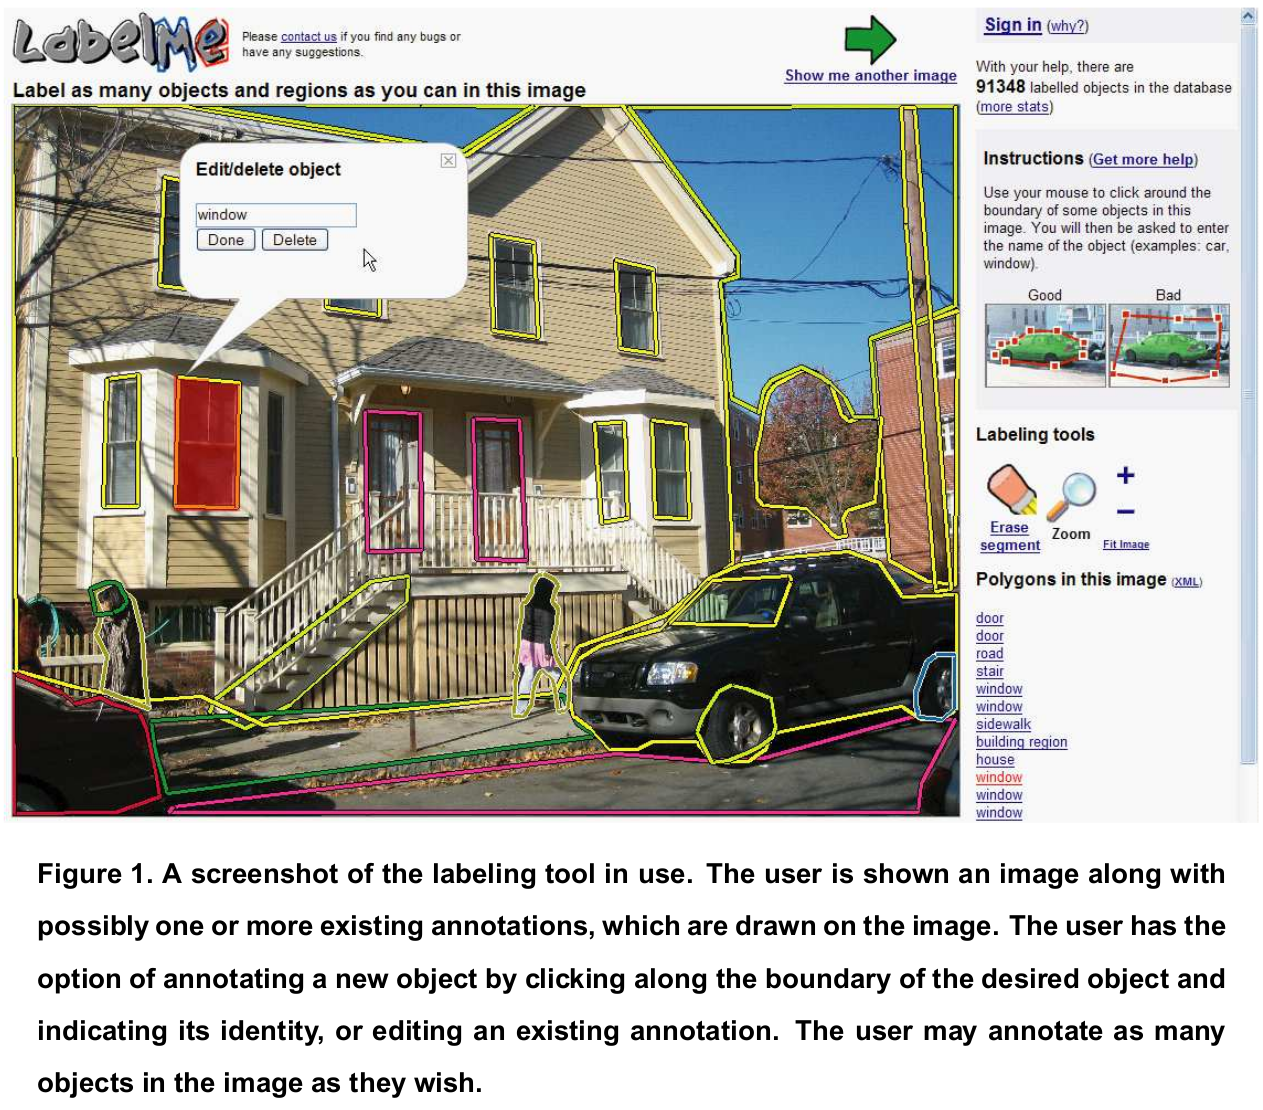
\includegraphics[width=\textwidth]{image-segmentation/labelme-interface}

\end{frame}

\begin{frame}
  \frametitle{Machine learning for image segmentation}

  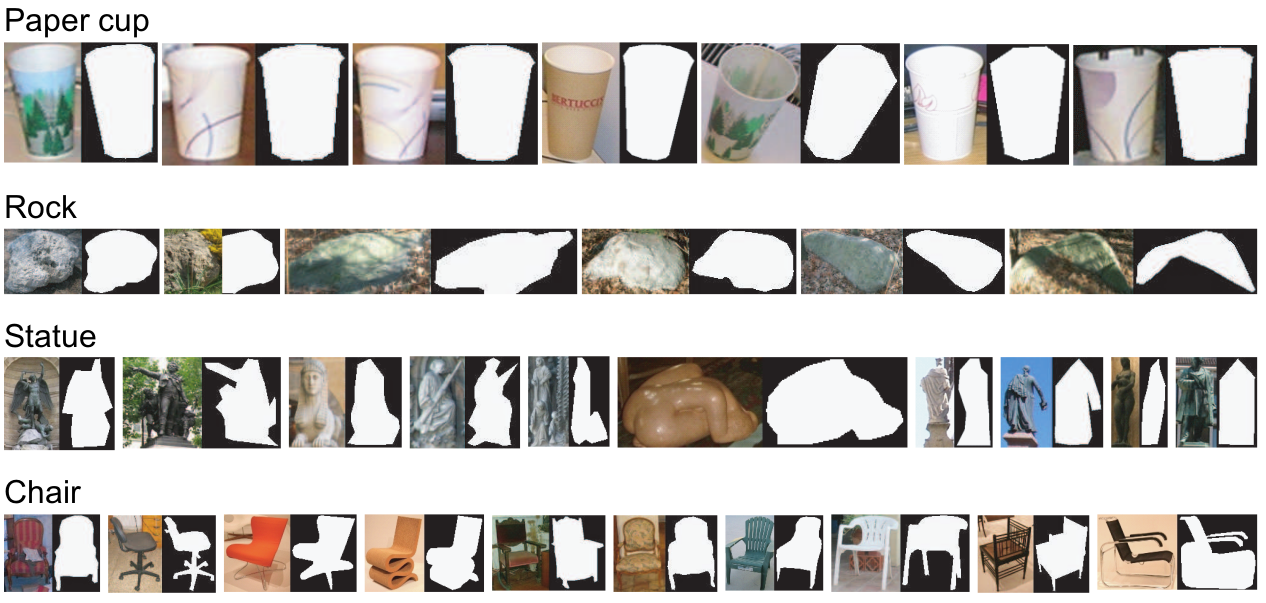
\includegraphics[width=\textwidth]{image-segmentation/labelme-examples}

  Russell {\it et al.} 2007.

  Q: What are the types/dimensions of $x,y,f$ in this example?

\end{frame}



\begin{frame}
  \frametitle{Machine learning for spam filtering (Gmail)}

  
\includegraphics[height=2in]{spam-filtering/screenshot-gmail-spam}
  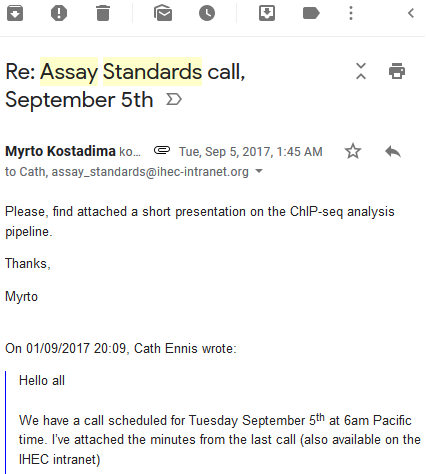
\includegraphics[height=2in]{spam-filtering/screenshot-inbox-message}

  Want: $f$(email message)$\in\{0,1\}$ -- binary classification, spam=1
  or not=0.

\end{frame}


\begin{frame}
  \frametitle{Machine learning for translation (google books)}

  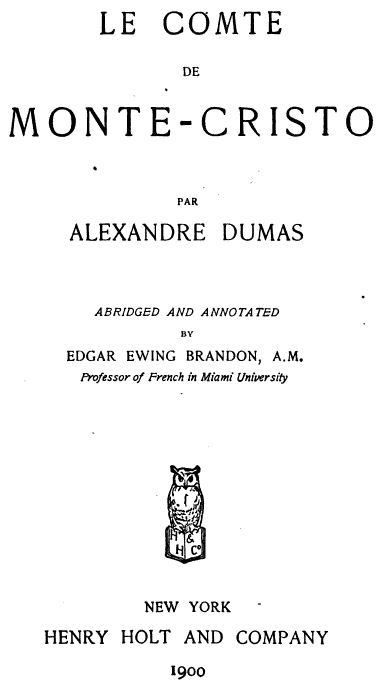
\includegraphics[height=3in]{translation/monte-cristo-french-title}
  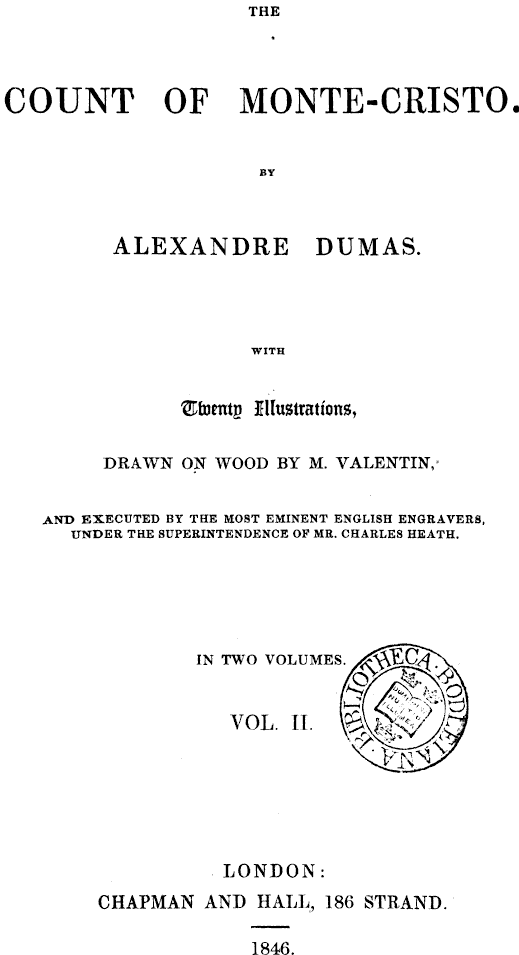
\includegraphics[height=3in]{translation/monte-cristo-english-title}

\end{frame}

\begin{frame}
  \frametitle{Machine learning for translation (google translate)}

  
  Want: $f$(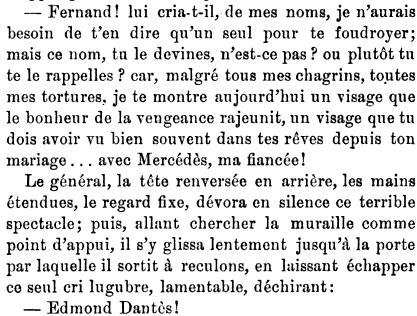
\includegraphics[width=0.5\textwidth]{translation/monte-cristo-french}) =
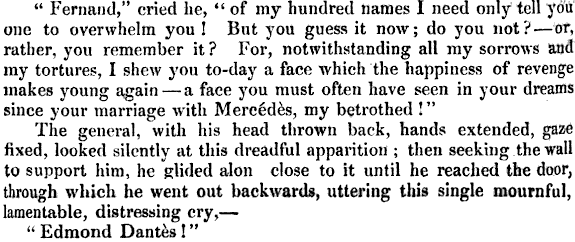
\includegraphics[width=0.8\textwidth]{translation/monte-cristo-english}

\end{frame}

\begin{frame}
  \frametitle{Machine learning for medical diagnosis}

\parbox{0.49\textwidth}{
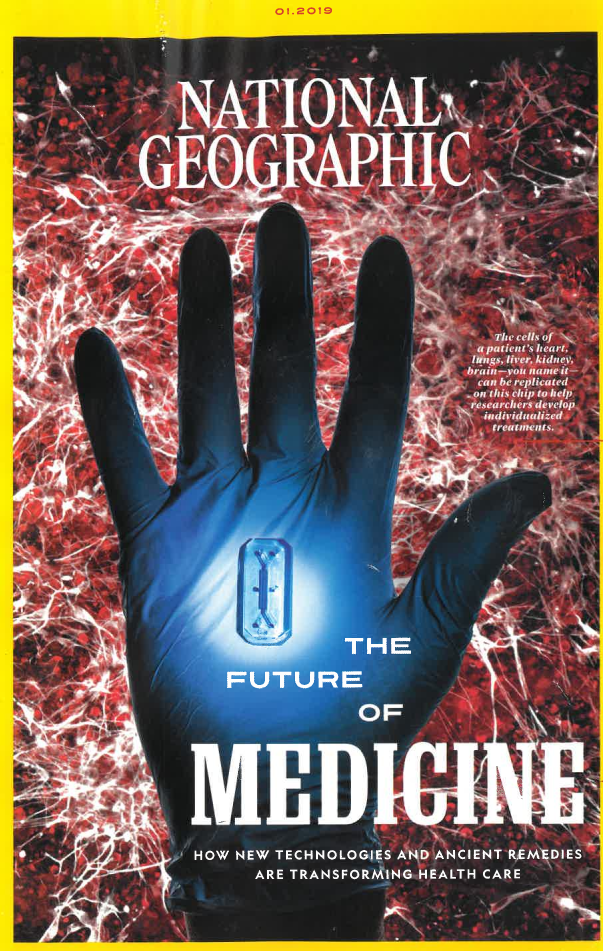
\includegraphics[height=0.9\textheight]{retinal-scans/national-geographic-medicine-cover}
}
\parbox{0.49\textwidth}{
f(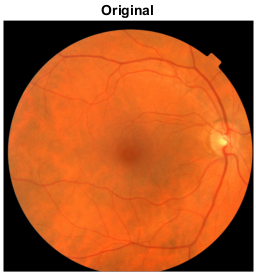
\includegraphics[width=0.5\textwidth]{retinal-scans/national-geographic-medicine-retina})=
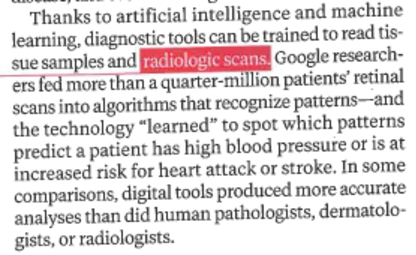
\includegraphics[width=0.5\textwidth]{retinal-scans/national-geographic-medicine-paragraph})
}

\end{frame}

\section{Demonstrating and avoiding overfitting in regression}
 
\begin{frame}
  \frametitle{Machine learning algorithms in practice}

  To learn a good prediction function for any of these problems (and
  any other problems you encounter in your work) you should
  \begin{itemize}
  \item First gather a data set that you will use to train/test the
    machine learning algorithms, typically a CSV file with rows for
    observations and columns for features.
  \item Use K-fold Cross-Validation to repeatedly divide the
    observations into train/test sets. Use the train set to learn
    machine learning model parameters, and use the test set to
    estimate prediction error.
  \item Try a variety of different learning algorithms (e.g. linear
    models, random forests, boosting, neural networks, support vector
    machines, ...), because you don't know which one will result in
    most accurate predictions for any given data set. 
  \item Each learning algorithm has different hyper-parameters which
    control complexity/regularization/overfitting, and typically must
    be chosen by the user (you) by dividing the train data into
    subtrain/validation sets. Use the hyper-parameter which is
    best with respect to the held-out validation set.
  \end{itemize}
  
\end{frame}

\begin{frame}
  \frametitle{Goal of this section: demonstrate overfitting}
  \begin{itemize}
  \item The goal of supervised machine learning is to get accurate
    predictions on new/unseen/held-out test data.
  \item Any machine learning algorithm is prone to overfit, which
    means providing better predictions on the train/subtrain set than
    on a held-out validation/test set. (BAD)
  \item To learn a model which does NOT overfit (GOOD), you need to
    first divide your train set into subtrain/validation sets.
  \item Code for figures in this section:
    \url{https://github.com/tdhock/2020-yiqi-summer-school/blob/master/figure-overfitting.R}
  \end{itemize}
\end{frame}

\begin{frame}
  \frametitle{Three different data sets/patterns}
  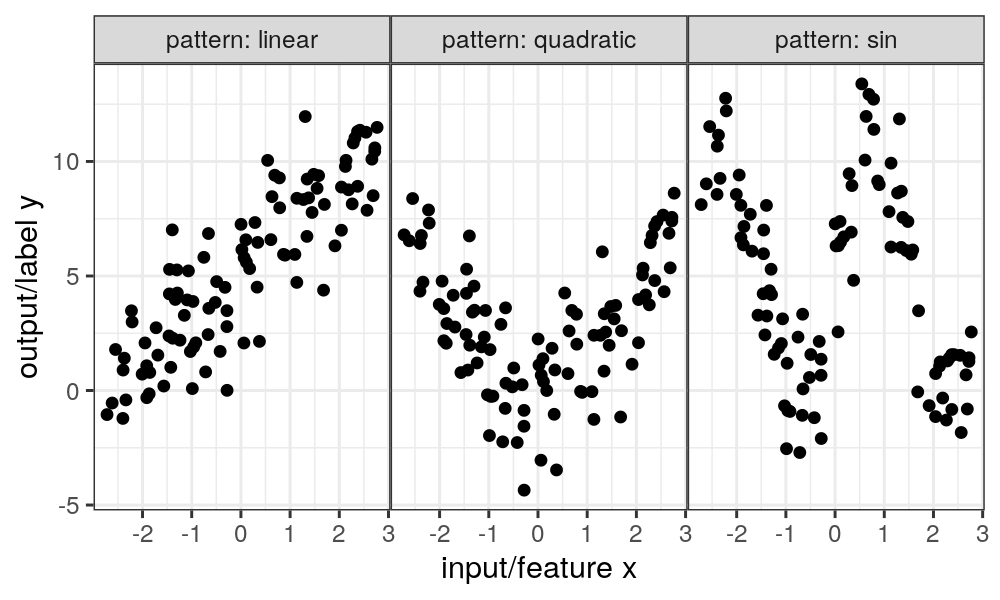
\includegraphics[width=\textwidth]{figure-overfitting-data}

  \begin{itemize}
   \item We illustrate this using a single input/feature
    $x\in\mathbb R$.
  \item We use a regression problem with outputs $y\in\mathbb R$.
  \item Goal is to learn a function $f(x)\in\mathbb R$.
  \end{itemize}
\end{frame}

\begin{frame}
  \frametitle{Illustration of 4-fold cross-validation}
  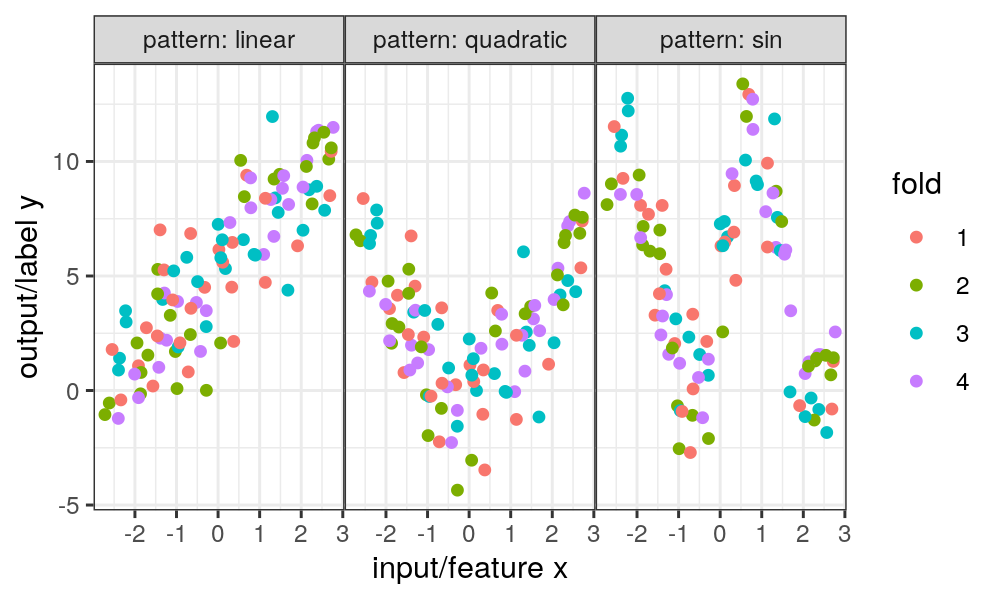
\includegraphics[width=\textwidth]{figure-overfitting-data-folds}

  Randomly assign each observation a fold ID from 1 to 4.
  
\end{frame}

\begin{frame}
  \frametitle{Illustration of subtrain/validation split}
  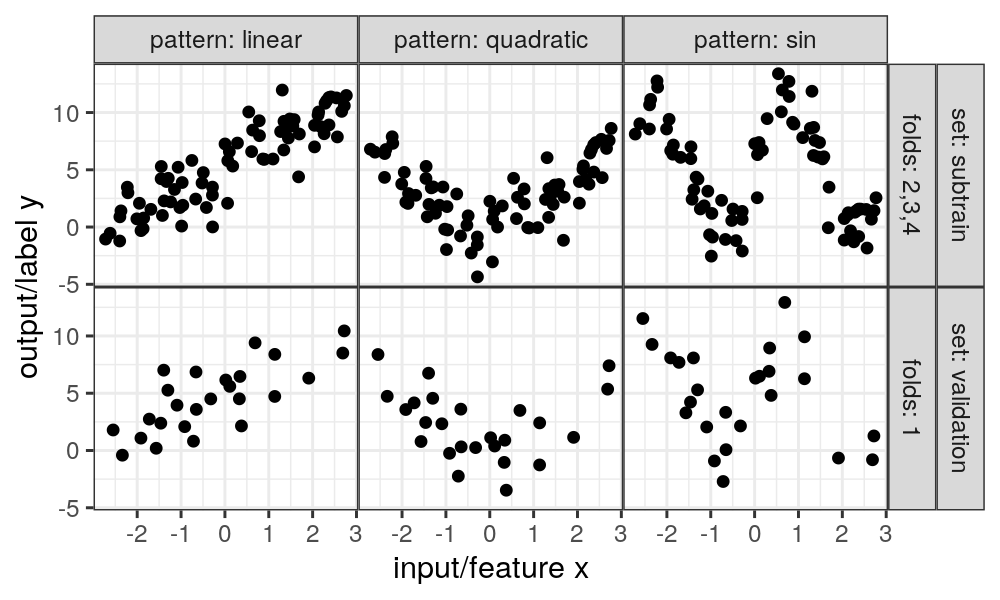
\includegraphics[width=\textwidth]{figure-overfitting-data-sets}

  \begin{itemize}
  \item For validation fold 1, all observations with that fold ID are
    considered the validation set.
  \item All other observations are considered the subtrain set.
  \end{itemize}
\end{frame}

\begin{frame}
  \frametitle{How to do this in practice? Use R with an IDE}
  \begin{itemize}
  \item Machine learning model training/evaluation is easy to code in
    programming languages which support vectors/matrices.
  \item I recommend using R because it has so many useful packages
    (each one for a different machine learning model/algorithm).
  \item Download R at \url{https://cloud.r-project.org/}
  \item If you already use Emacs (classic text editor), I recommend
    using R inside Emacs Speaks Statistics, which is a great
    Interactive Development Environment (IDE) for R
    \url{http://ess.r-project.org/} Also see my screencasts about ESS,
    \url{https://www.youtube.com/playlist?list=PLwc48KSH3D1Onsed66FPLywMSIQmAhUYJ}
  \item Otherwise, I recommend using RStudio, which is another popular
    IDE for R
    \url{https://rstudio.com/products/rstudio/download}
  \end{itemize}
\end{frame}

\begin{frame}[fragile]
  \frametitle{CSV data tables for machine learning}
  \begin{itemize}
  \item One row for each observation.
  \item One column for the output/label/y (in regression the label is a real
    number, in classification the label is a class/category).
  \item The other columns should be inputs/features/X that will be used
    to predict the corresponding output/label/y.
  \end{itemize}

  Example:
  \url{https://raw.githubusercontent.com/tdhock/2020-yiqi-summer-school/master/data_linear.csv}

\begin{verbatim}
               x            y
  1: -1.40694802  0.933196336
  2: -0.76725660  3.832773444
  3:  0.43712018  4.202983135
  4:  2.44924674 13.089055084
...
\end{verbatim}
\end{frame}

\begin{frame}[fragile,fragile]
  \frametitle{Download CSV data and get file names into R}

  Download a copy of the github repo to get these data sets
  \url{https://github.com/tdhock/2020-yiqi-summer-school/archive/master.zip}

Set working directory to the downloaded repo:

\begin{verbatim}
> setwd("~/teaching/2020-yiqi-summer-school")
> getwd()
[1] "/home/tdhock/teaching/2020-yiqi-summer-school"
\end{verbatim}

  Get a character vector of CSV data file names:
  
\begin{verbatim}
> csv.vec <- Sys.glob("data_*.csv")
> csv.vec
[1] "data_linear.csv"    "data_quadratic.csv"
[3] "data_sin.csv"      
\end{verbatim}

\end{frame}

\begin{frame}[fragile,fragile]
  \frametitle{Read each CSV data file into R}
\begin{verbatim}
sim.data.list <- list()
for(csv in csv.vec){
  pattern <- gsub("data_|.csv", "", csv)
  sim.dt <-  data.table::fread(csv)
  set.seed(1) # for reproducibility.
  fold.vec <- sample(rep(1:4, l=nrow(sim.dt)))
  sim.data.list[[pattern]] <- data.table::data.table(
    pattern, sim.dt, fold=factor(fold.vec))
} # combine into a single data table:
sim.data <- do.call(rbind, sim.data.list)
\end{verbatim}

  \begin{itemize}
  \item \texttt{gsub} removes prefix/suffix from CSV file name.
  \item \texttt{data.table::fread} gets CSV data from file into R.
  \item \texttt{set.seed} used to get consistent/reproducible results from the
    pseudo-random number generator (\texttt{sample}).
  \item \texttt{data.table::fun} means use \texttt{fun} from
    \texttt{data.table} package, install it via
    \texttt{install.packages("data.table")}
  \end{itemize}
\end{frame}

\begin{frame}[fragile]
  \frametitle{Result of reading CSV data into R}
  Result is:

\begin{verbatim}
> sim.data
     pattern          x          y fold
  1:  linear -1.4069480  0.9331963    4
  2:  linear -0.7672566  3.8327734    3
  3:  linear  0.4371202  4.2029831    1
  4:  linear  2.4492467 13.0890551    2
  5:  linear -1.7899084  2.0791987    3
 ---                                   
296:     sin  1.7838530  4.0502991    1
297:     sin -0.2683533 -0.1097264    1
298:     sin -0.5394955 -0.5539398    1
299:     sin  1.8652215 -0.2262517    4
300:     sin  0.6295997  8.8124249    4
\end{verbatim}
  
\end{frame}

\begin{frame}[fragile]
  \frametitle{Assign each observation to subtrain/validation set}

\begin{verbatim}
validation.fold <- 1
sim.data[, set := ifelse(
  fold==validation.fold, "validation", "subtrain")]
> sim.data
     pattern          x          y fold        set
  1:  linear -1.4069480  0.9331963    4   subtrain
  2:  linear -0.7672566  3.8327734    3   subtrain
  3:  linear  0.4371202  4.2029831    1 validation
  4:  linear  2.4492467 13.0890551    2   subtrain
  5:  linear -1.7899084  2.0791987    3   subtrain
 ---                                              
296:     sin  1.7838530  4.0502991    1 validation
297:     sin -0.2683533 -0.1097264    1 validation
298:     sin -0.5394955 -0.5539398    1 validation
299:     sin  1.8652215 -0.2262517    4   subtrain
300:     sin  0.6295997  8.8124249    4   subtrain
\end{verbatim}
  
\end{frame}

\begin{frame}[fragile]
  \frametitle{Neural network with one hidden layer, 20 hidden units}

  Use for loops to fit different neural network models for each data
  set and number of iterations. 

\begin{verbatim}
maxit.values <- 10^seq(0, 4)
pattern.values <- c("linear", "quadratic", "sin")
for(i in maxit.values)for(p in pattern.values){
  pattern.data <- sim.data[pattern==p]
  fit <- nnet::nnet(
    y ~ x,
    pattern.data[set=="subtrain"],
    size=20,     #hidden units
    linout=TRUE, #for regression
    maxit=i)     #max number of iterations
...
\end{verbatim}

\end{frame}


\begin{frame}
  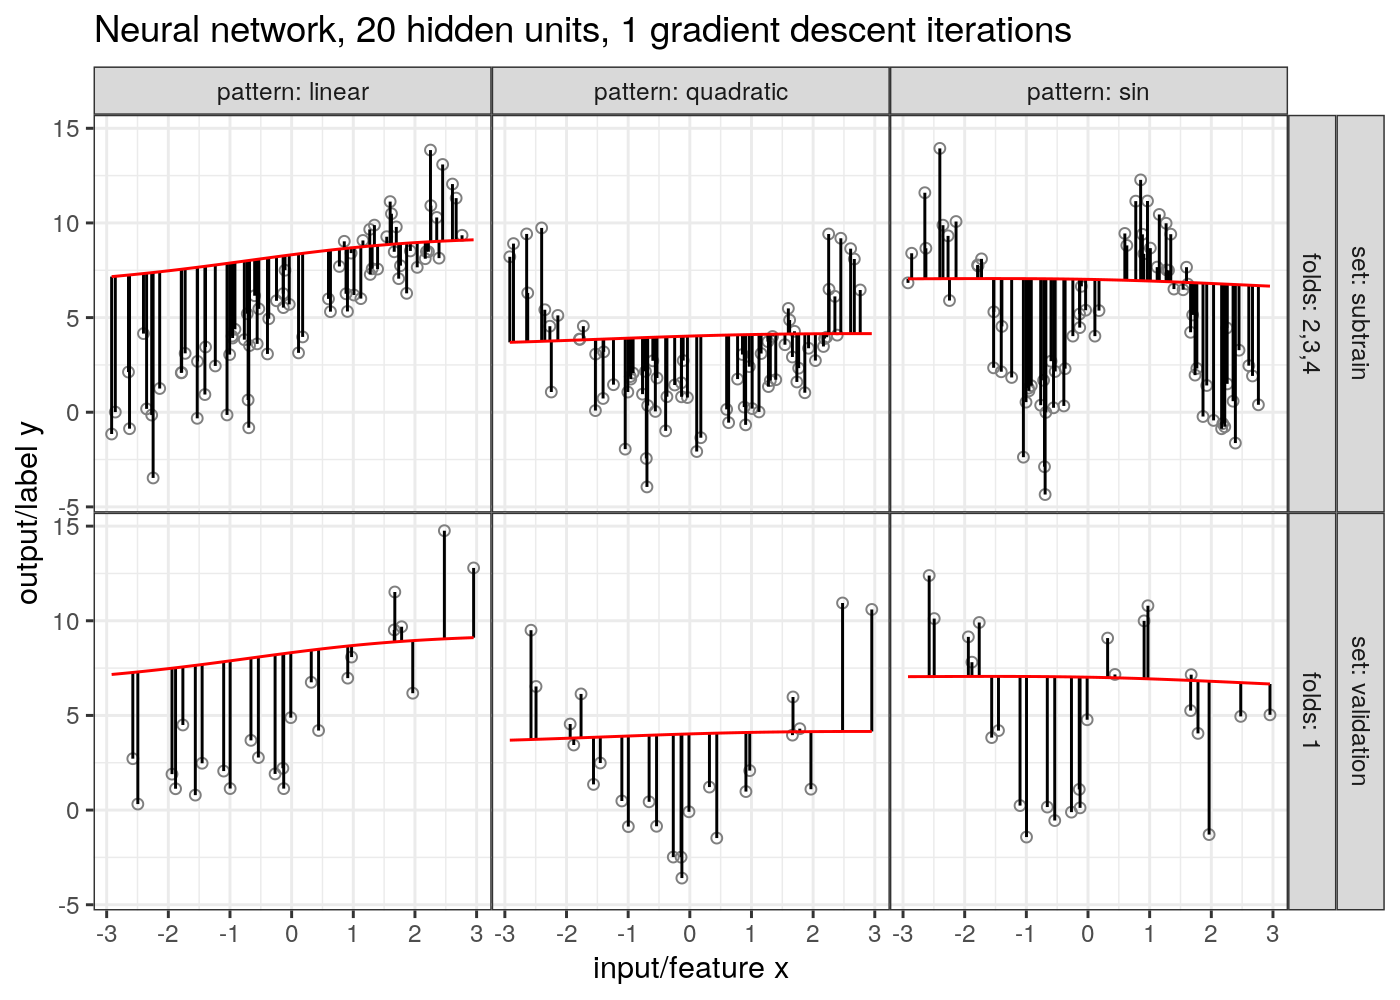
\includegraphics[width=\textwidth]{figure-overfitting-pred-units=20-maxit=1.png}
\end{frame}


\begin{frame}
  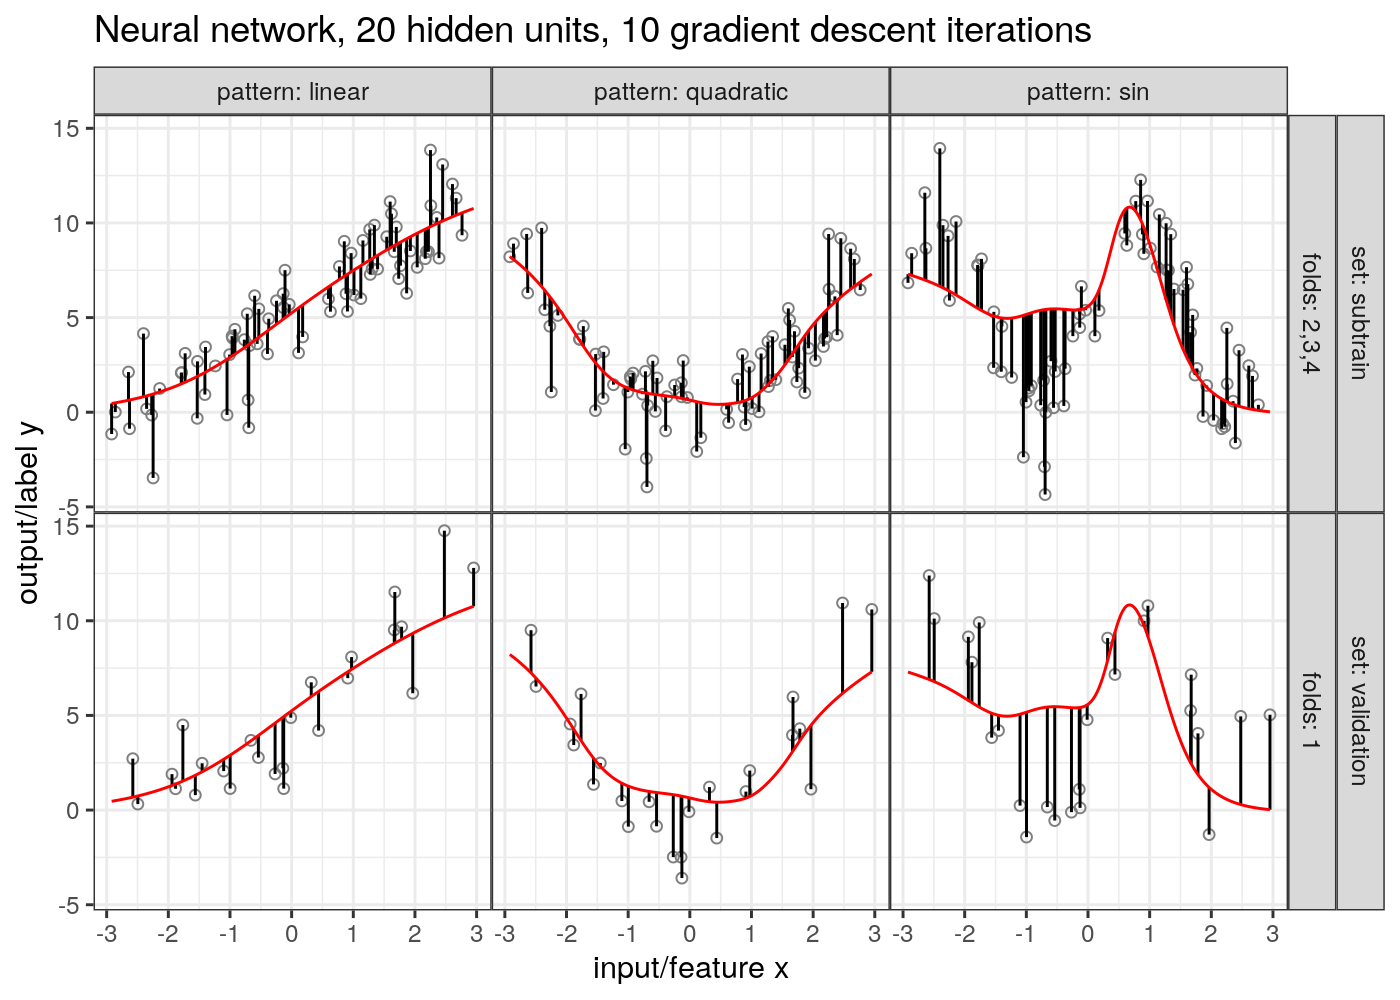
\includegraphics[width=\textwidth]{figure-overfitting-pred-units=20-maxit=10.png}
\end{frame}


\begin{frame}
  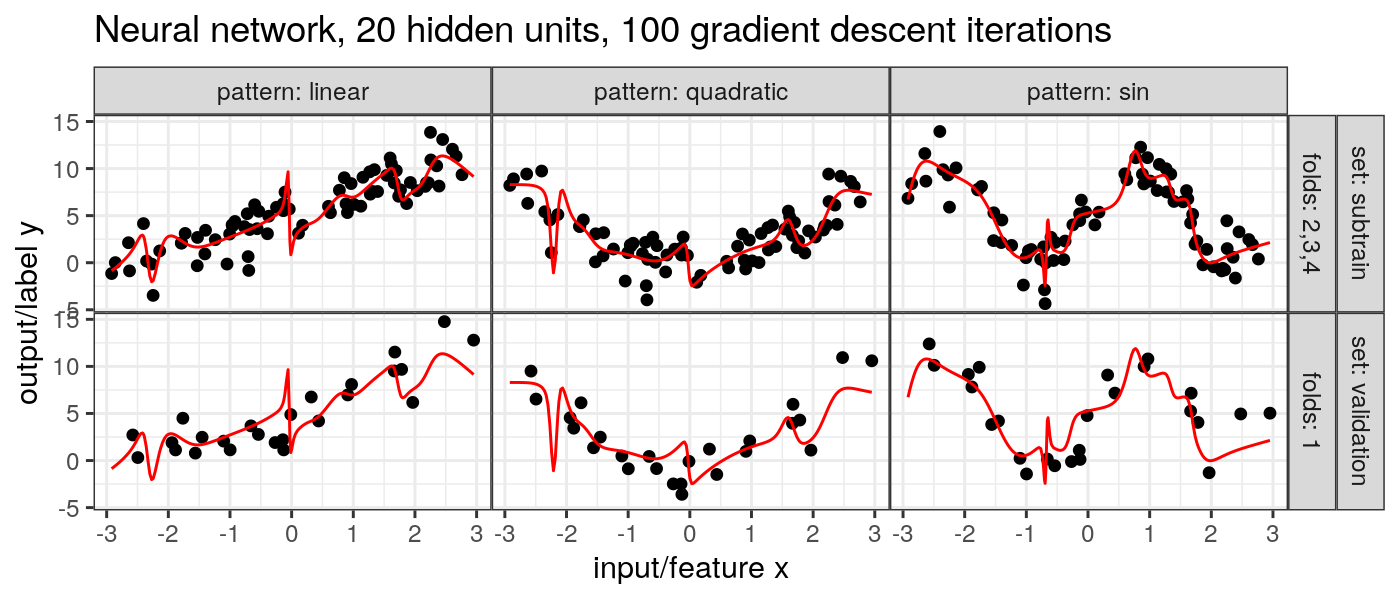
\includegraphics[width=\textwidth]{figure-overfitting-pred-units=20-maxit=100.png}
\end{frame}


\begin{frame}
  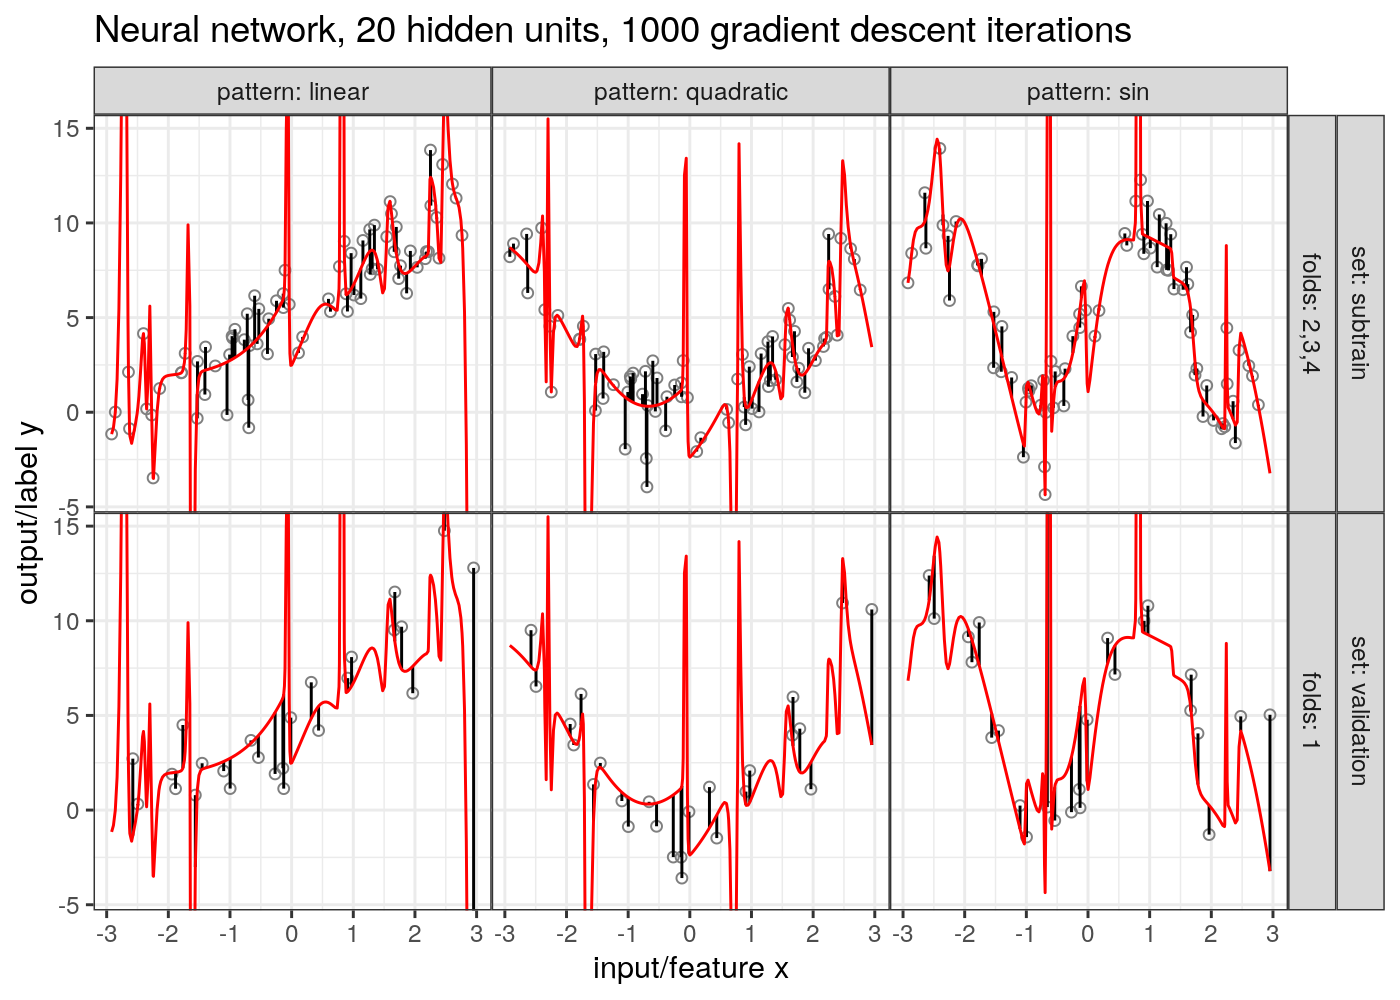
\includegraphics[width=\textwidth]{figure-overfitting-pred-units=20-maxit=1000.png}
\end{frame}


\begin{frame}
  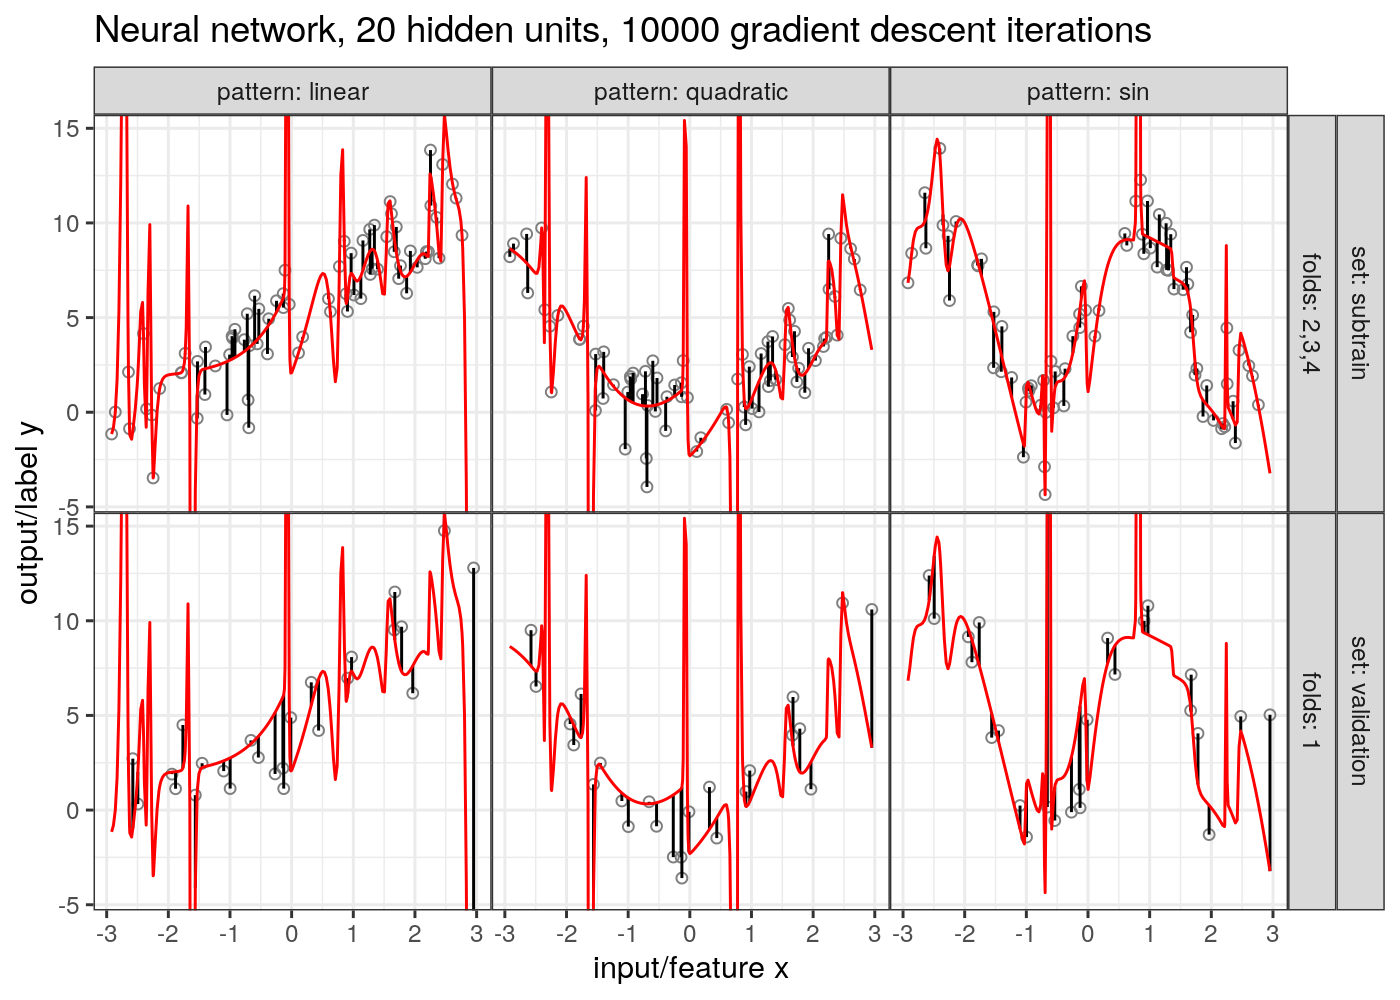
\includegraphics[width=\textwidth]{figure-overfitting-pred-units=20-maxit=10000.png}
\end{frame}


\begin{frame}
  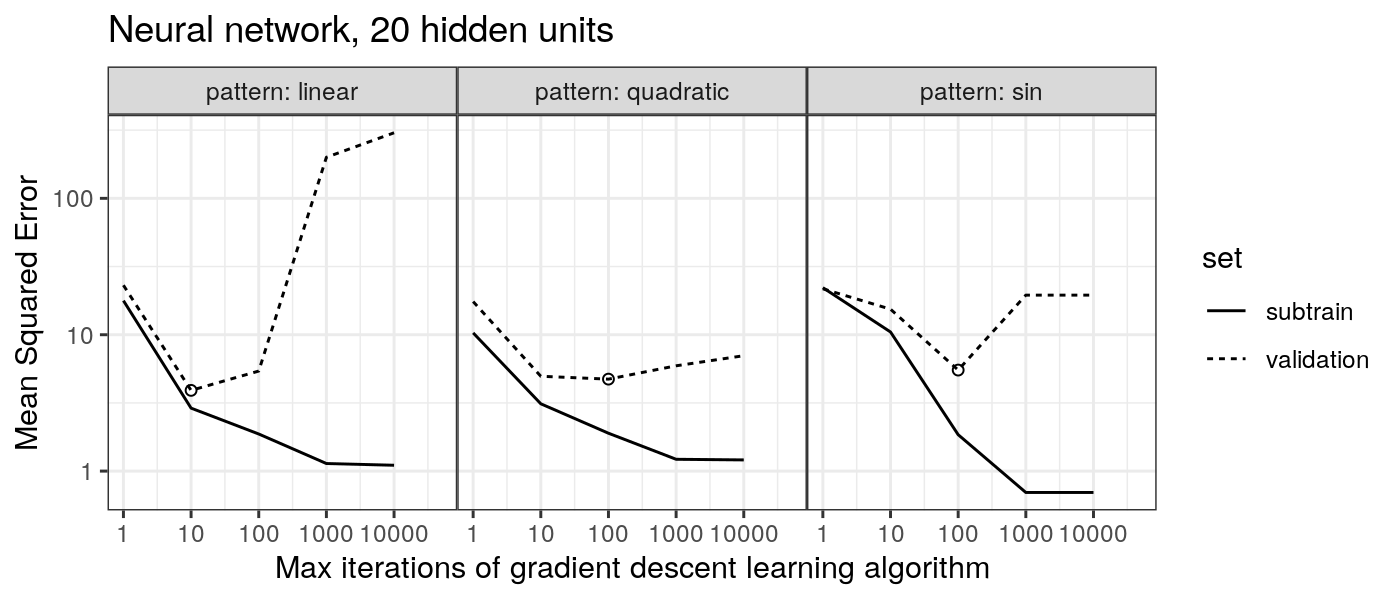
\includegraphics[width=\textwidth]{figure-overfitting-data-loss-20.png}
\end{frame}



\begin{frame}
  \frametitle{Overfitting}
  \begin{itemize}
  \item Happens when subtrain error/loss decreases but validation error
    increases (as a function of some hyper-parameter)
  \item Here the hyper-parameter is the number of iterations of
    gradient descent, and overfitting starts after 10--100 iterations.
  \item To maximize prediction accuracy you need to choose a
    hyper-parameter with minimal validation error/loss.
  \item This optimal hyper-parameter will depend on the data set.
  \item In this case that means choosing 10 iterations for the linear
    data set, and 100 iterations for the quadratic/sin data sets.
  \end{itemize}
\end{frame}

\begin{frame}[fragile]
  \frametitle{Computing subtrain/validation loss curves}

\begin{verbatim}
...
  pattern.data[, pred.y := as.numeric(predict(
    fit, pattern.data))]
  loss.dt.list[[paste(pattern, maxit)]] <- data.table(
    pattern=p, maxit=i, pattern.data[, .(
      mse=mean((pred.y-y)^2)), by=set])
}
loss.dt <- do.call(rbind, loss.dt.list)
\end{verbatim}
  
\begin{verbatim}
      pattern        set maxit         mse
 1:    linear   subtrain     1  17.7785881
 2:    linear validation     1  23.0575528
...
29:       sin   subtrain 10000   0.6970455
30:       sin validation 10000  19.5051785
\end{verbatim}
\end{frame}


\begin{frame}
  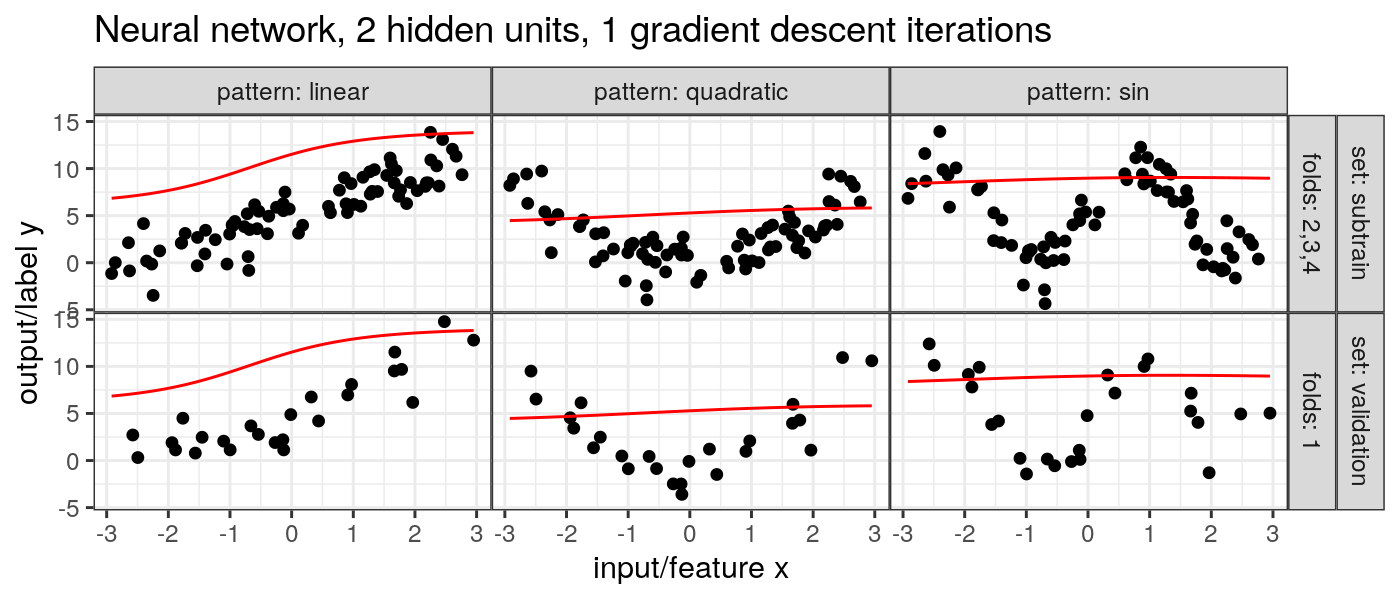
\includegraphics[width=\textwidth]{figure-overfitting-pred-units=2-maxit=1.png}
\end{frame}


\begin{frame}
  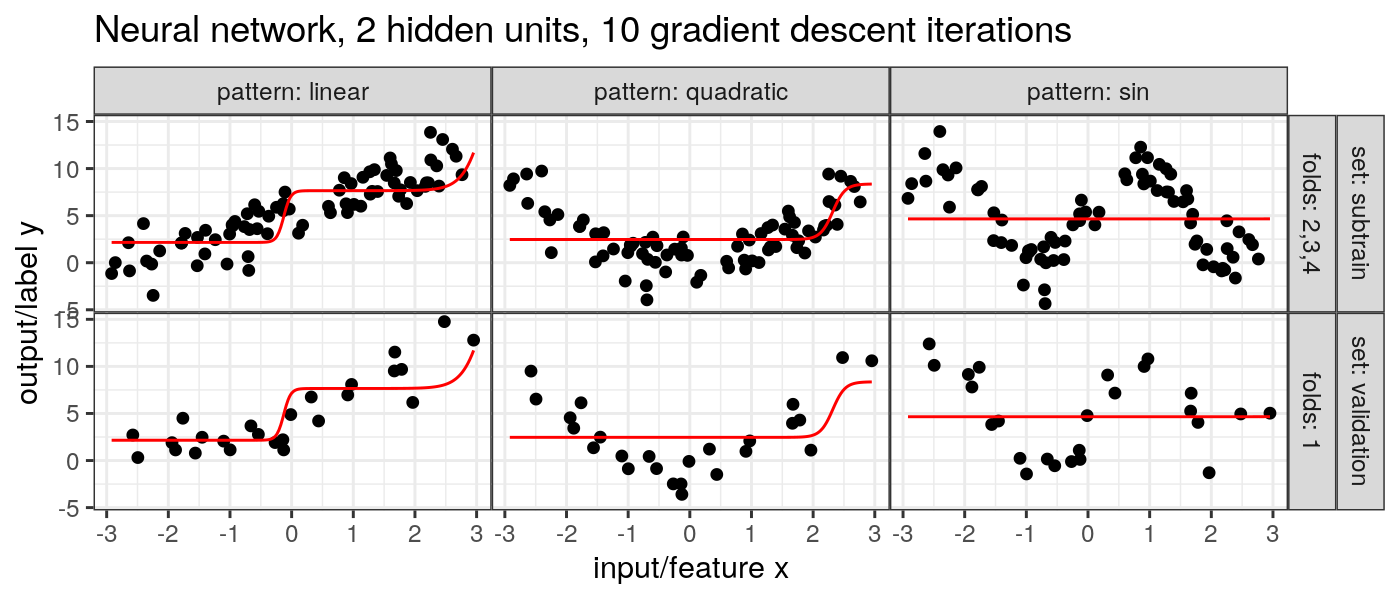
\includegraphics[width=\textwidth]{figure-overfitting-pred-units=2-maxit=10.png}
\end{frame}


\begin{frame}
  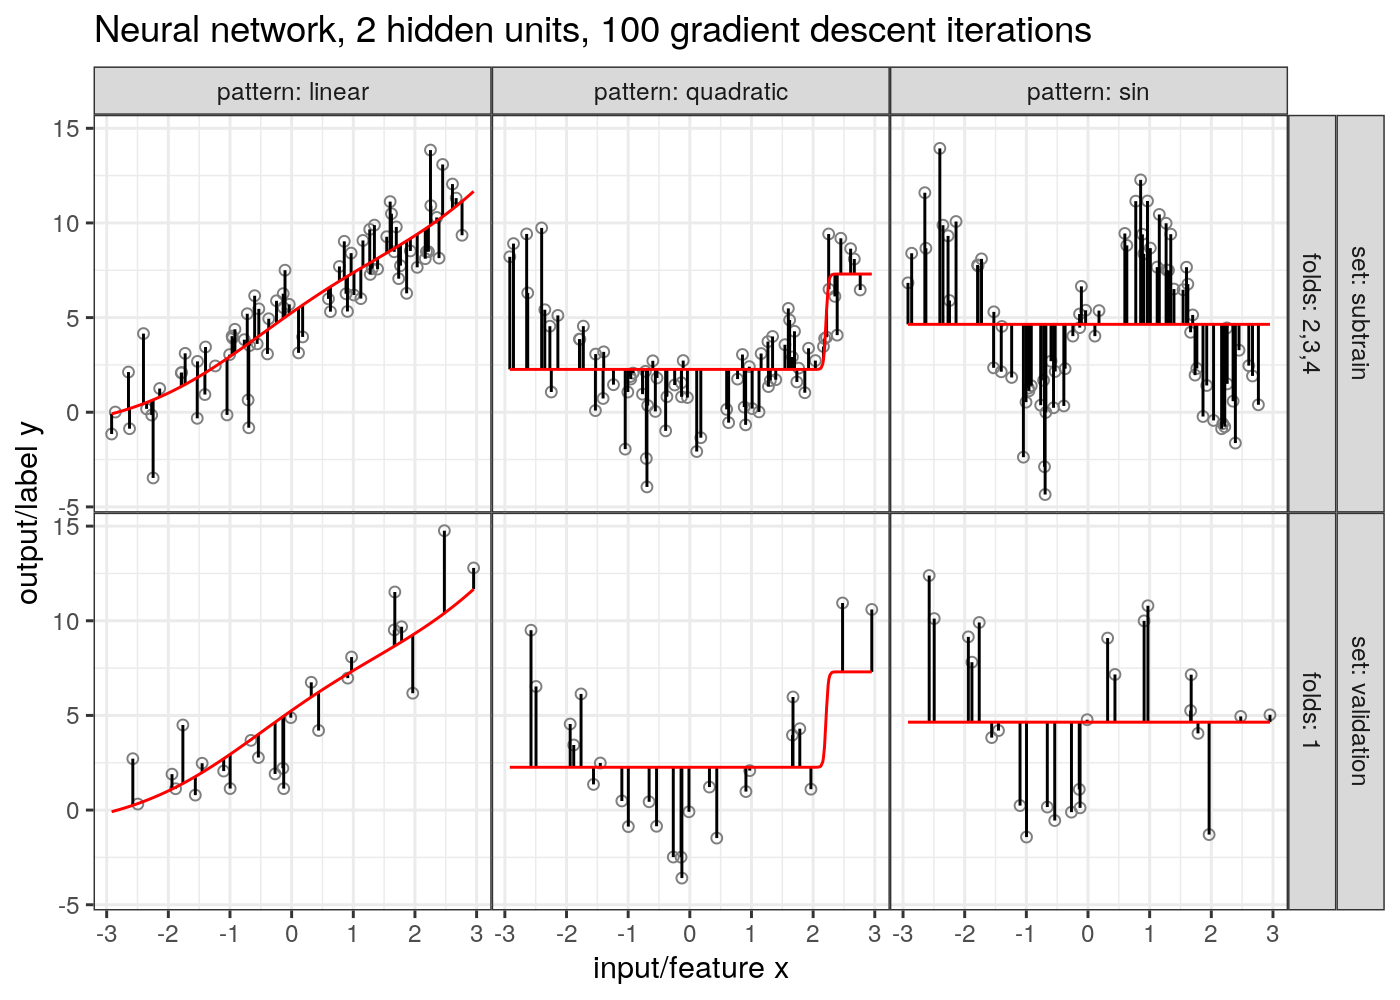
\includegraphics[width=\textwidth]{figure-overfitting-pred-units=2-maxit=100.png}
\end{frame}


\begin{frame}
  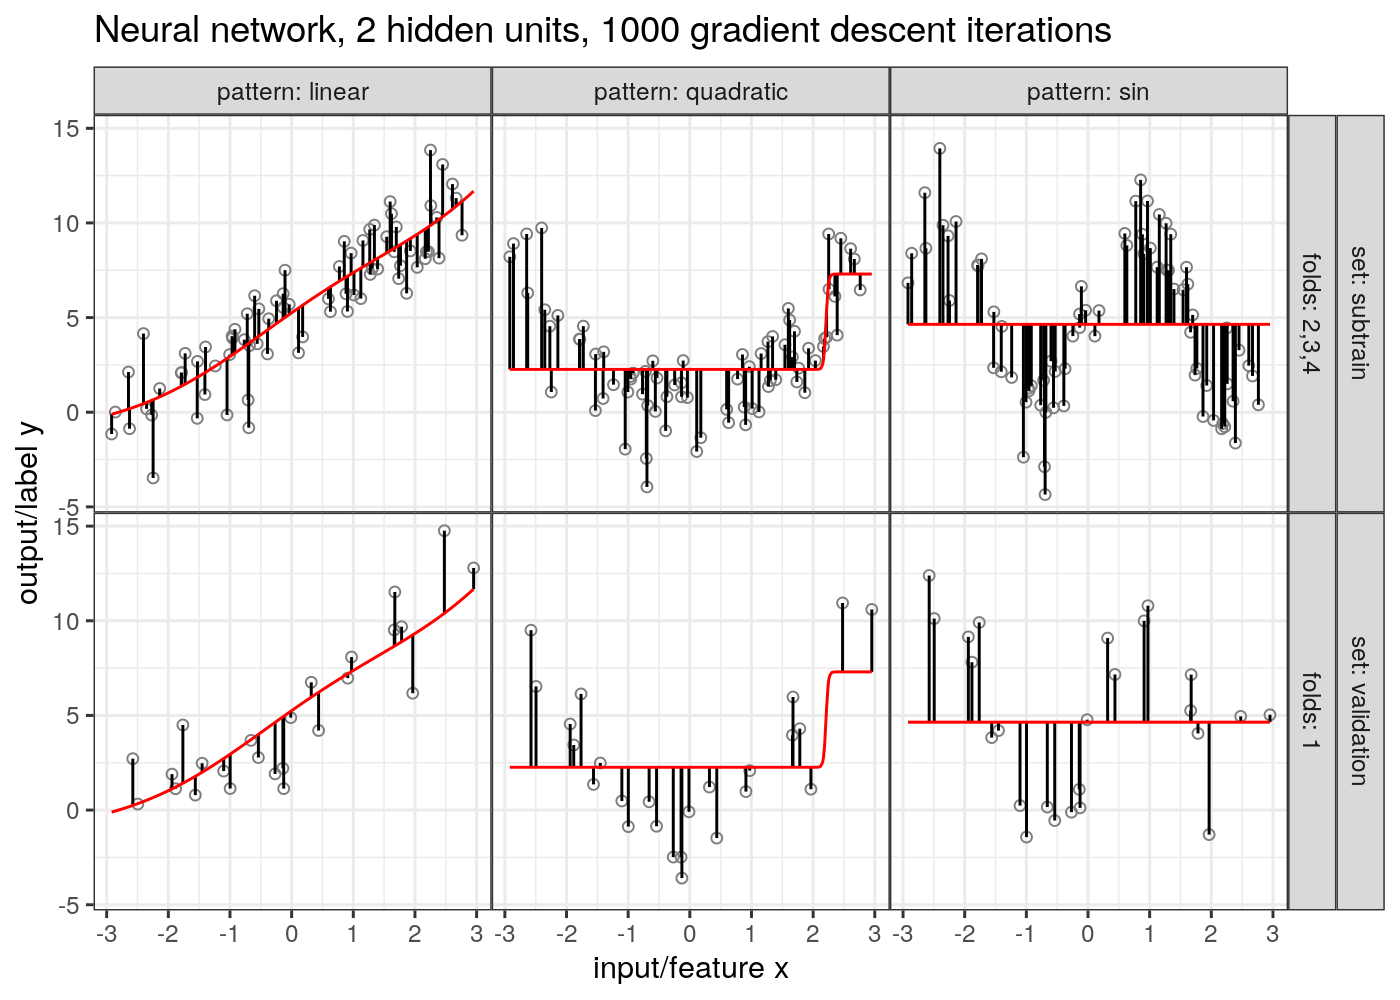
\includegraphics[width=\textwidth]{figure-overfitting-pred-units=2-maxit=1000.png}
\end{frame}


\begin{frame}
  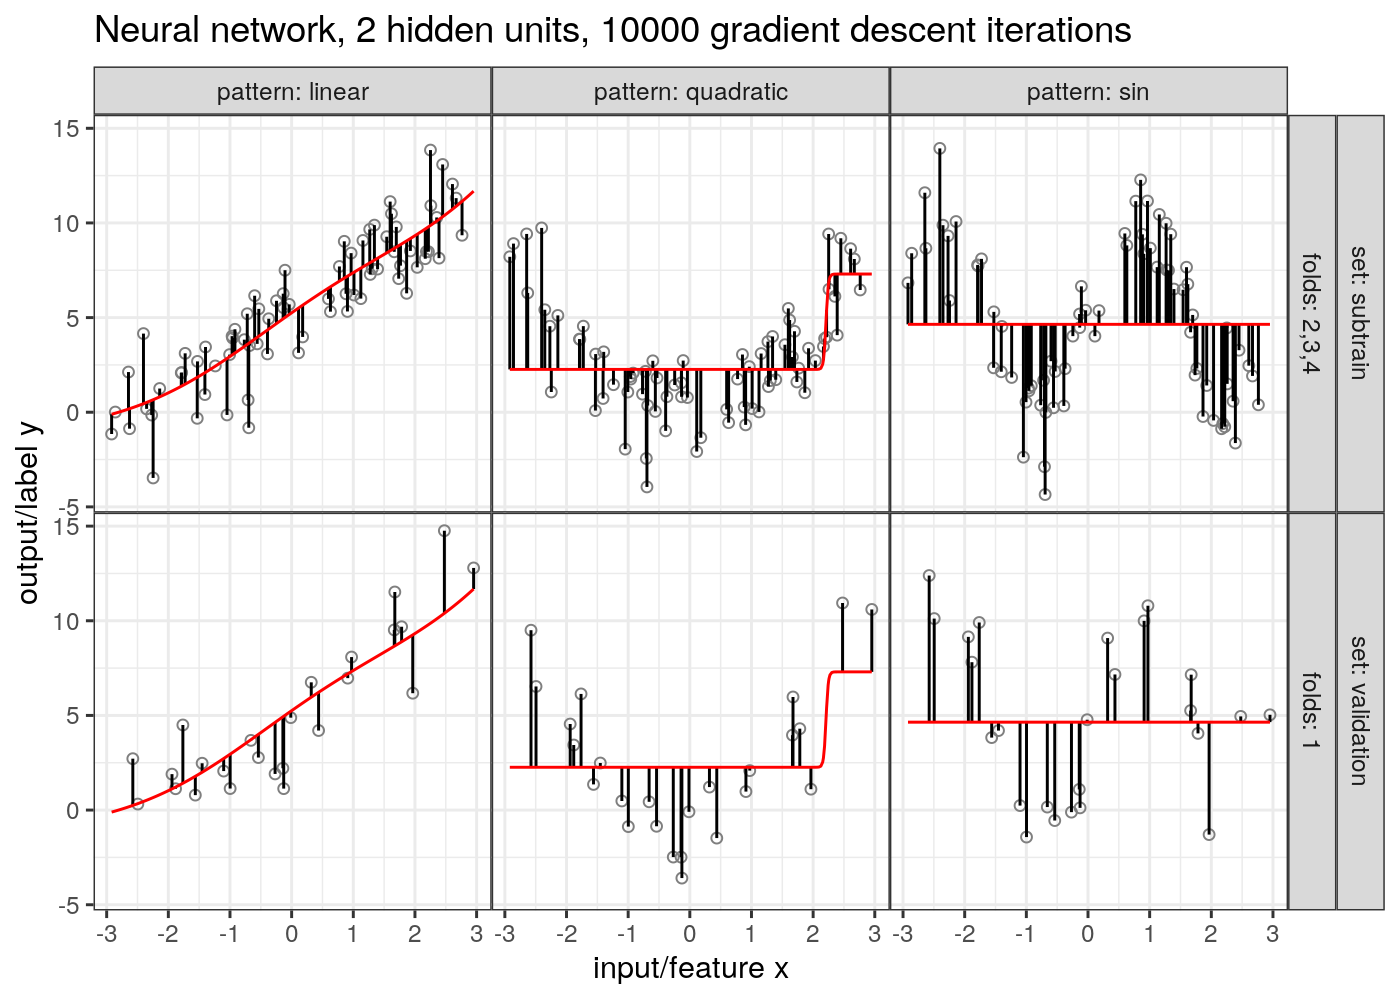
\includegraphics[width=\textwidth]{figure-overfitting-pred-units=2-maxit=10000.png}
\end{frame}


\begin{frame}
  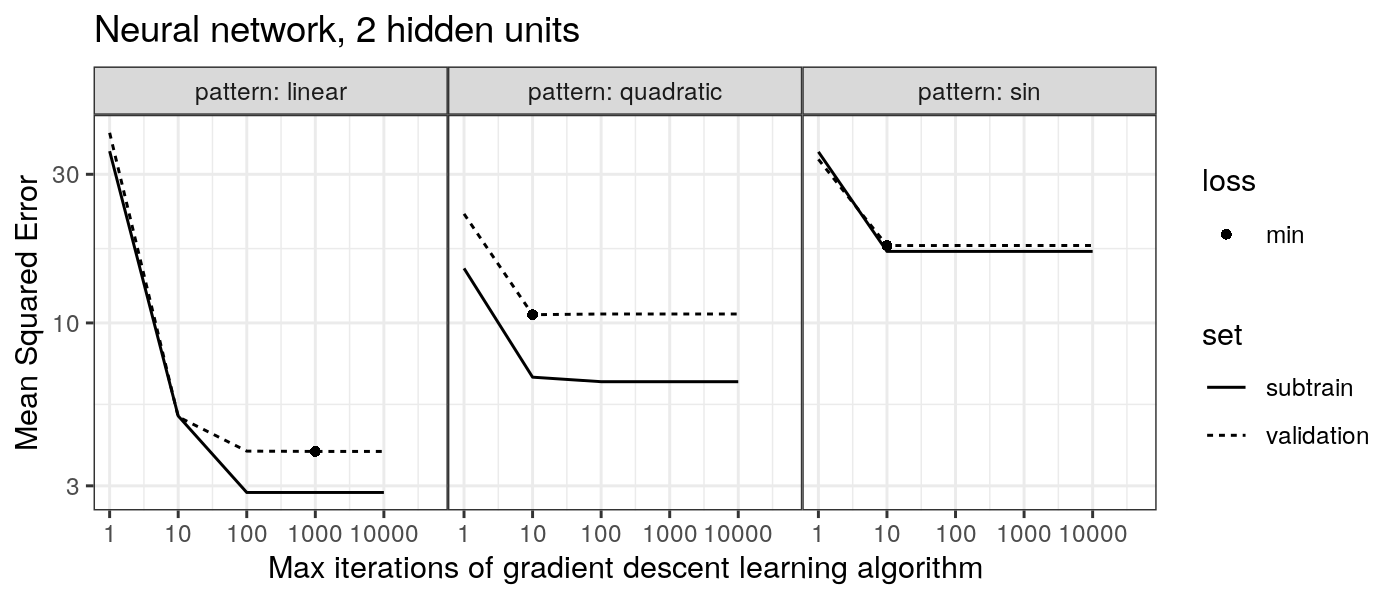
\includegraphics[width=\textwidth]{figure-overfitting-data-loss-2.png}
\end{frame}



\begin{frame}[fragile]
  \frametitle{How does the neural network predict/learn?}

  \begin{eqnarray*}
    \text{hidden units: }\ h_j &=& \sigma(w_j x + b_j) \\
    \text{predicted output: }\  \texttt{o} = \hat y &=& \sum_{j=1}^u v_j h_j + \beta
  \end{eqnarray*}

  \begin{itemize}
  \item $x\in\mathbb R$ is the input/feature (\texttt{i1} in R notation below).
  \item $\sigma:\mathbb R\rightarrow [0,1]$ is the sigmoid activation
    function, $\sigma(z)=(1+e^{-z})^{-1}$.
  \item $h_j\in[0,1]$ are $u$ hidden units, e.g. $u\in\{20, 2\}$ (\texttt{h1},\texttt{h2}).
  \item $w_j,b_j,v_j,\beta\in\mathbb R$ are the weights which are
    learned using gradient descent to minimize the squared error, e.g. for $u=2$:
  \end{itemize}

\begin{verbatim}
> coef(fit)
     b->h1     i1->h1      b->h2     i1->h2 
-40.770433  -2.636863 -20.719333   2.629485 
      b->o      h1->o      h2->o 
  4.643852  18.973225  28.348342 
\end{verbatim}
\end{frame}



\begin{frame}
  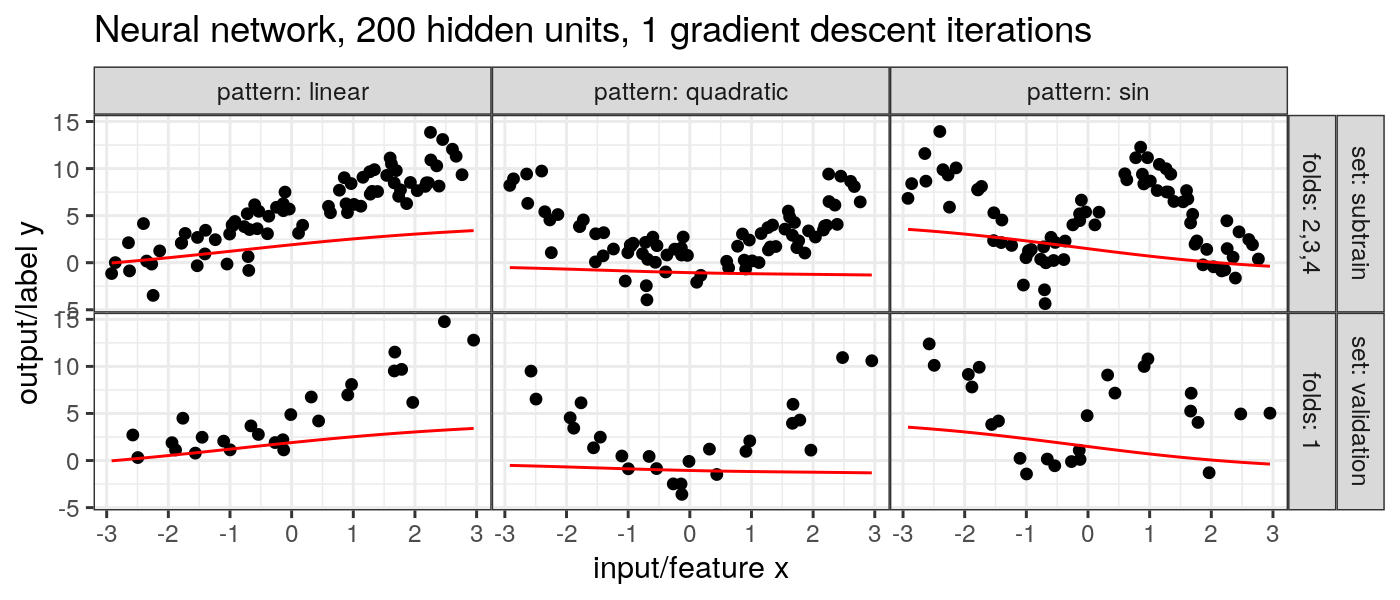
\includegraphics[width=\textwidth]{figure-overfitting-pred-units=200-maxit=1.png}
\end{frame}


\begin{frame}
  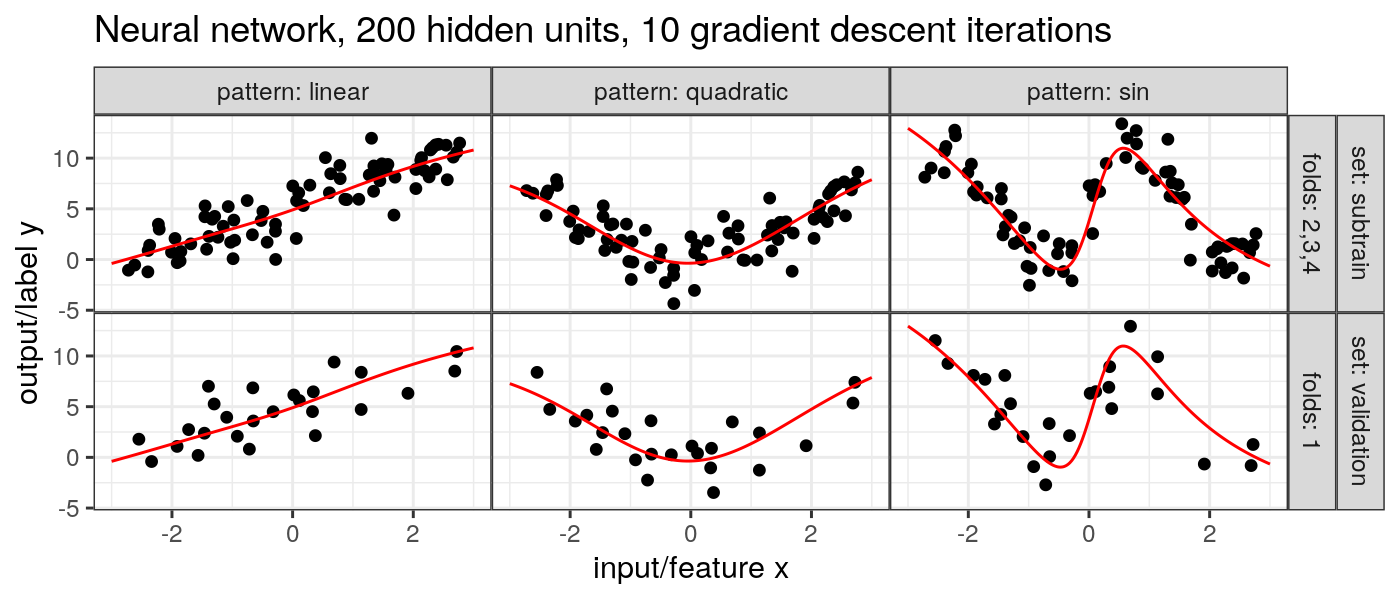
\includegraphics[width=\textwidth]{figure-overfitting-pred-units=200-maxit=10.png}
\end{frame}


\begin{frame}
  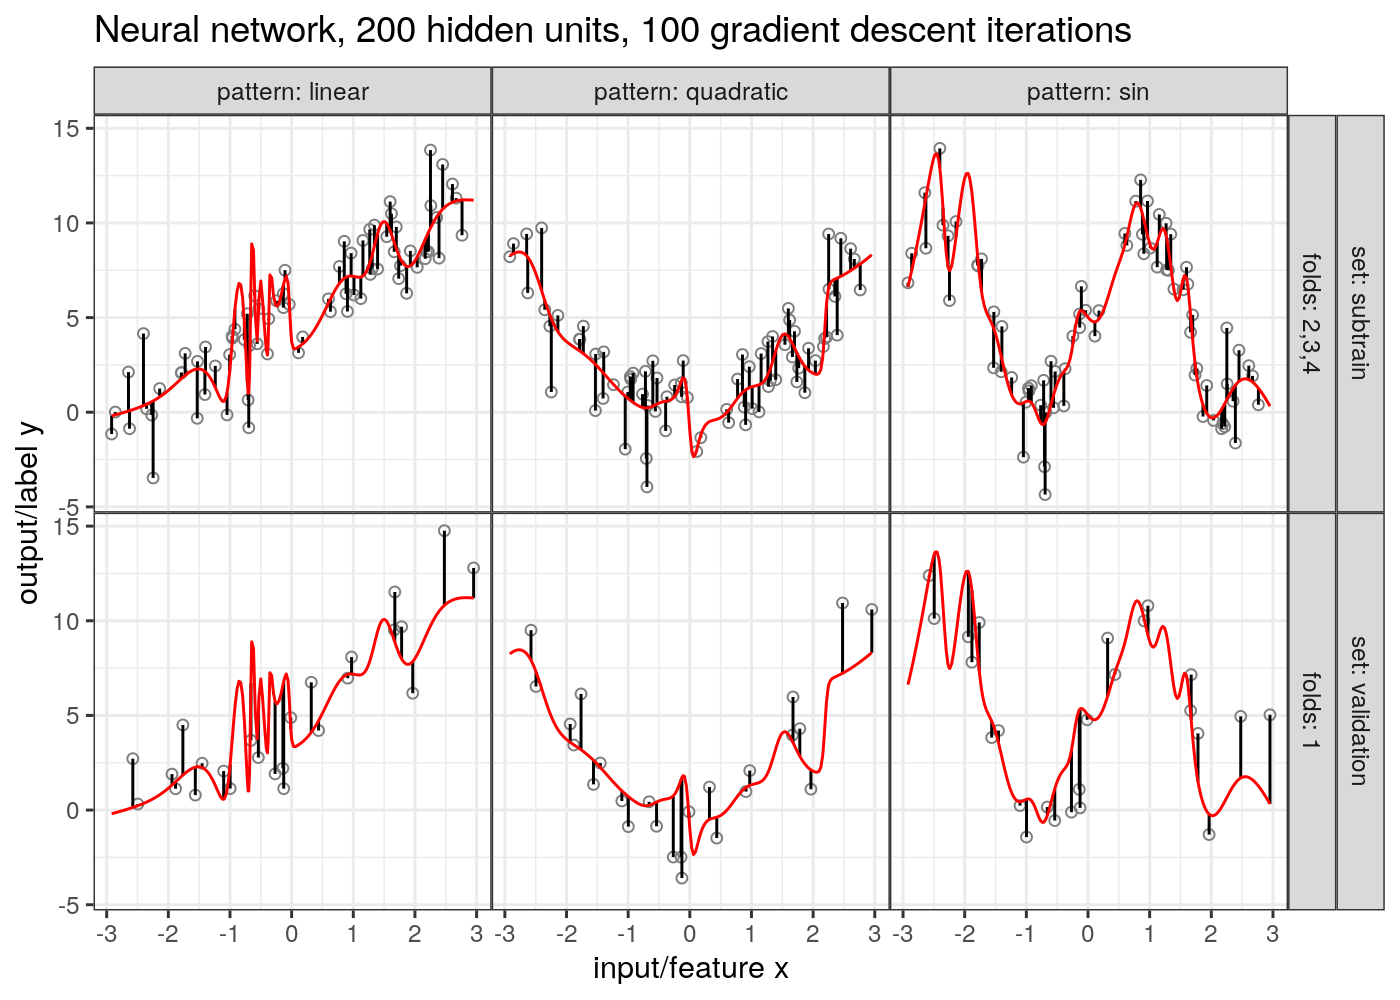
\includegraphics[width=\textwidth]{figure-overfitting-pred-units=200-maxit=100.png}
\end{frame}


\begin{frame}
  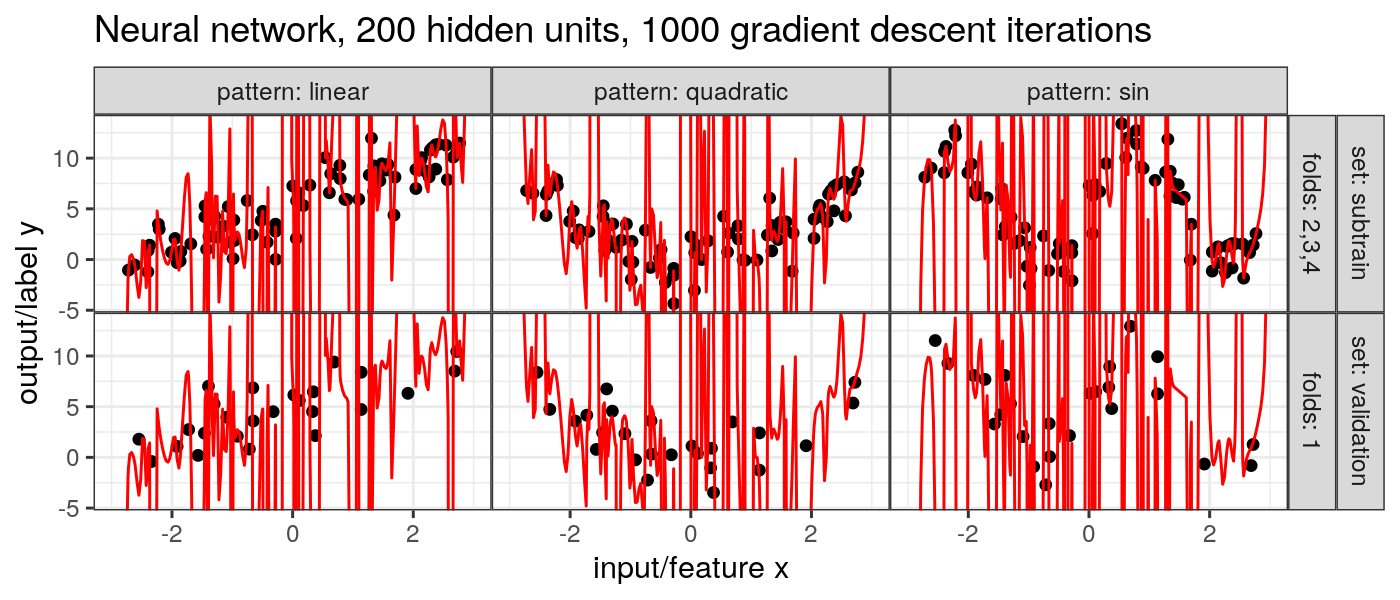
\includegraphics[width=\textwidth]{figure-overfitting-pred-units=200-maxit=1000.png}
\end{frame}


\begin{frame}
  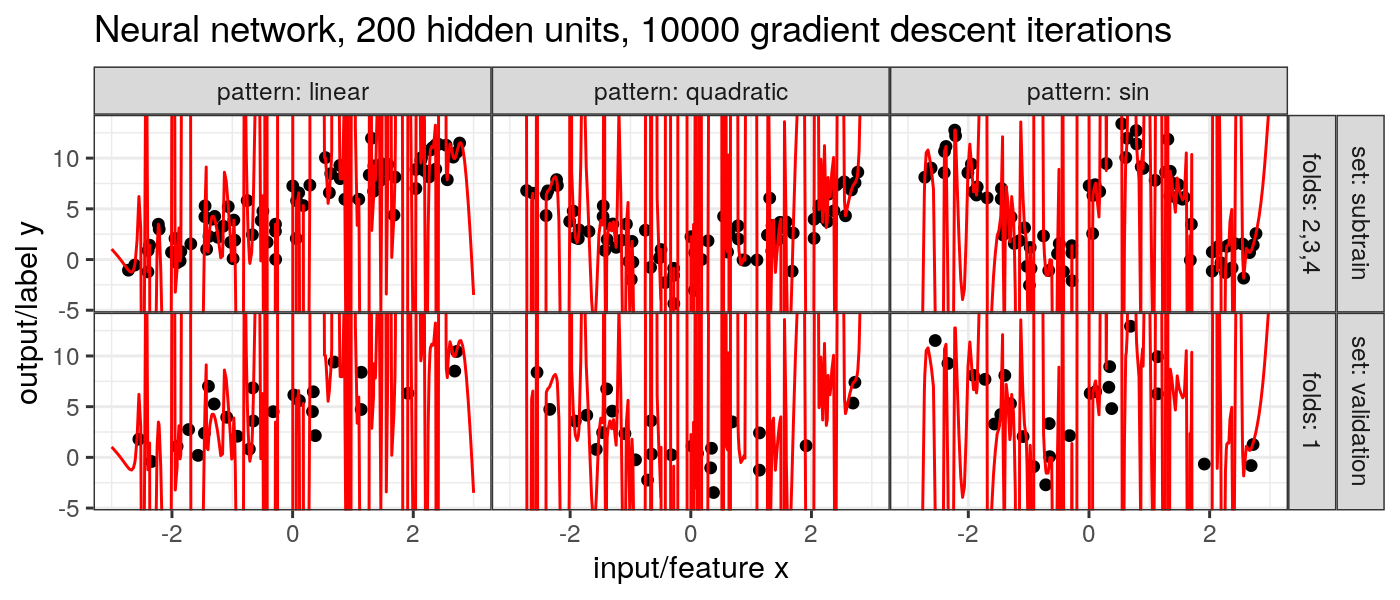
\includegraphics[width=\textwidth]{figure-overfitting-pred-units=200-maxit=10000.png}
\end{frame}


\begin{frame}
  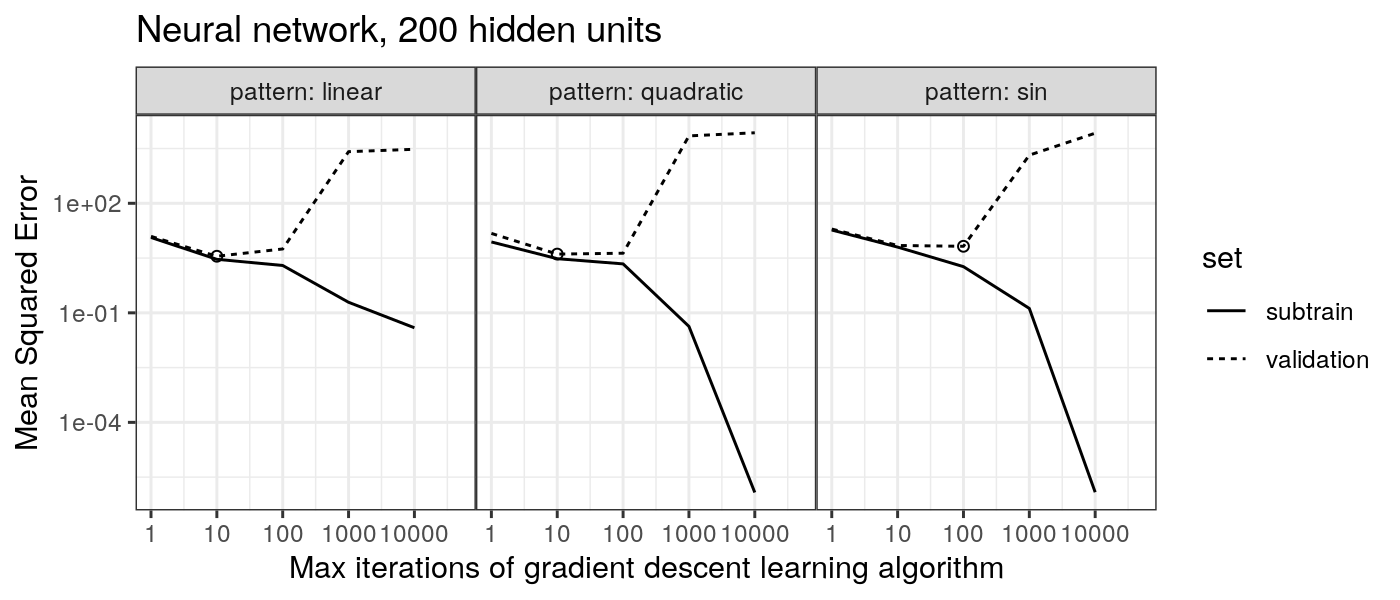
\includegraphics[width=\textwidth]{figure-overfitting-data-loss-200.png}
\end{frame}



\begin{frame}
  \frametitle{Comments on other model sizes}
  \begin{itemize}
  \item Model with 2 hidden units is less flexible: does not fit the subtrain
    data as well, and does not overfit as much.
  \item Model with 200 hidden units is more flexible: fits subtrain
    data even better, and overfits even more.
  \item Therefore model size / number of hidden units is also a
    hyper-parameter that can be used to control overfitting.
  \item R code is the same, just use \texttt{size=2} or 200 (or even
    better, I wrote a for loop over size values).
  \item Conclusion: you need to use a held-out validation set to
    choose the best values of hyper-parameters (e.g. number of
    iterations, hidden units).
  \end{itemize}
\end{frame}

\begin{frame}
  \frametitle{Minimizing over both hyper-parameters}

  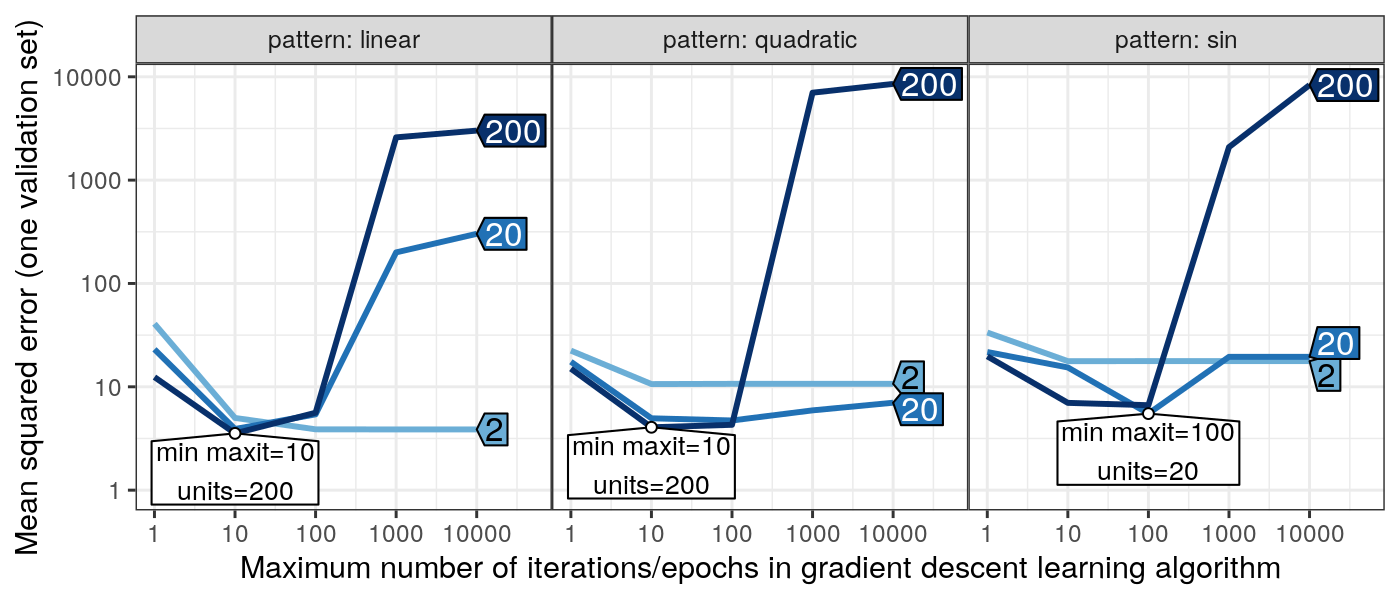
\includegraphics[width=\textwidth]{figure-overfitting-validation-only}
  
\end{frame}

\section{Inner and outer cross-validation}

\begin{frame}
  \frametitle{Machine learning algorithms in practice}

  \begin{itemize}
  \item Last section: we saw how to split the train set into
    subtrain/validation sets in order to tune hyper-parameters.
  \item This section: we use K-fold Cross-Validation to repeatedly
    divide the observations into train/test sets. Use the train set to
    learn machine learning model parameters, and use the test set to
    estimate prediction error. Important if you want to demonstrate
    that your algorithm is learning (providing accurate preditions on
    new/test data), and comparing different algorithms.
  \end{itemize}
  
\end{frame}

\begin{frame}
  \frametitle{Inner and outer cross-validation}

  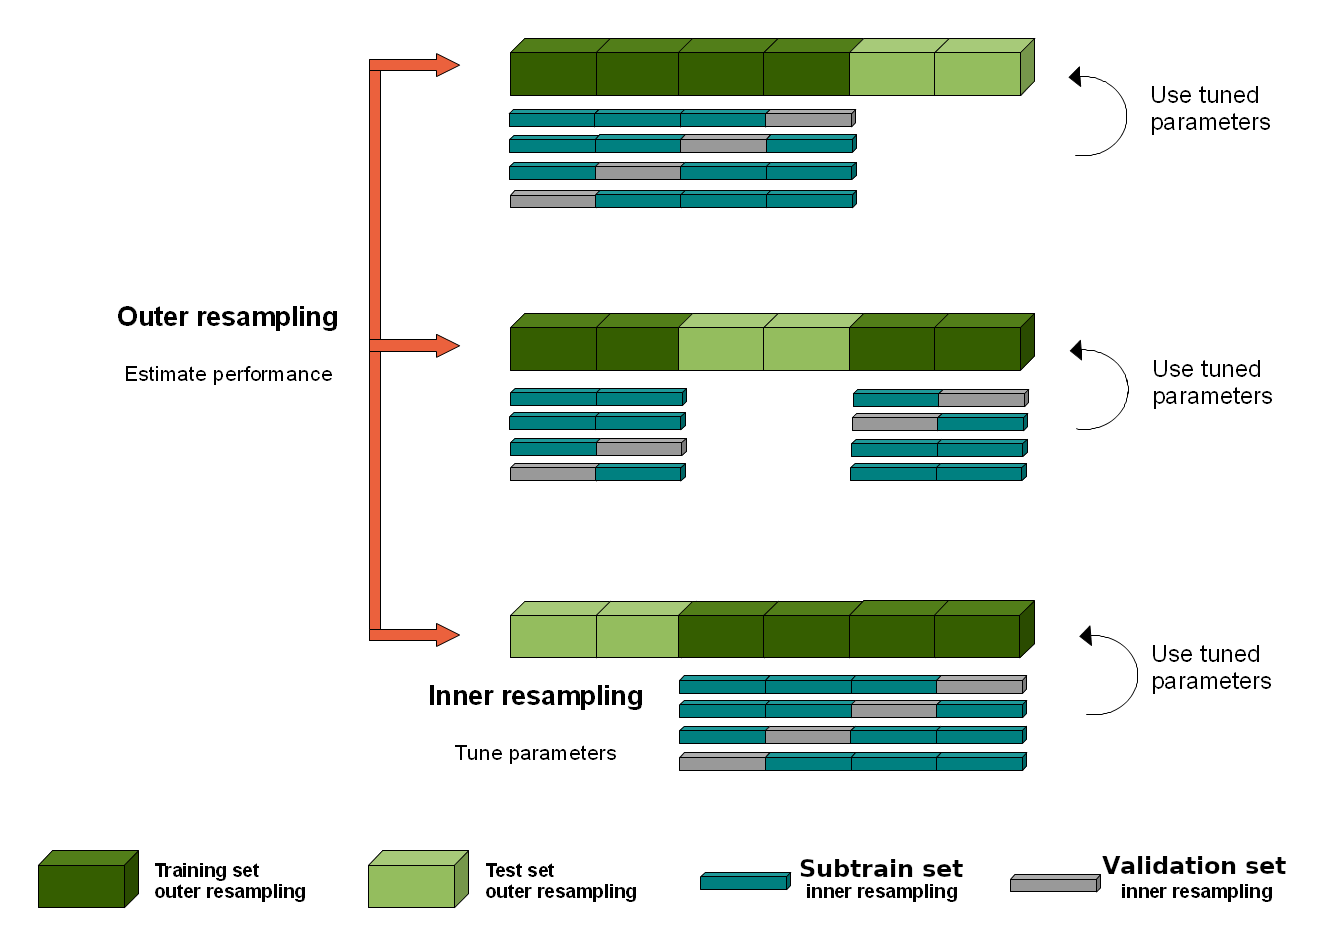
\includegraphics[width=\textwidth]{nested_resampling}

  {\scriptsize Source: \url{https://raw.githubusercontent.com/mlr-org/mlr3book/main/bookdown/images/nested_resampling.png}}
  
\end{frame}

\begin{frame}
  \frametitle{Outer cross-validation}

  \includegraphics[width=\textwidth]{figure-overfitting-cv-data-outer-folds}
  
\end{frame}

\begin{frame}
  \frametitle{Fix one outer fold = one train/test split}

  \includegraphics[width=\textwidth]{figure-overfitting-cv-data-test-fold-1.png}
  
\end{frame}

\begin{frame}
  \frametitle{Assign inner folds for one train set}

  \includegraphics[width=\textwidth]{figure-overfitting-cv-data-inner-folds-1.png}
  
\end{frame}

\begin{frame}
  \frametitle{Fix inner fold=1, subtrain/validation split}

  \includegraphics[width=\textwidth]{figure-overfitting-cv-data-inner-folds-1-1.png}  
\end{frame}

\begin{frame}
  \frametitle{Inner fold=2, another subtrain/validation split}

  \includegraphics[width=\textwidth]{figure-overfitting-cv-data-inner-folds-1-2.png}
\end{frame}

\begin{frame}
  \frametitle{Another subtrain/validation split}

  \includegraphics[width=\textwidth]{figure-overfitting-cv-data-inner-folds-1-3.png}
\end{frame}

\begin{frame}
  \frametitle{Average validation error over four splits (outer fold 1)}

  \includegraphics[width=\textwidth]{figure-overfitting-cv-data-median-mse-1.png}
\end{frame}

\begin{frame}
  \frametitle{Final models fit to entire train set using best hyper-parameters (outer fold 1)}

  \includegraphics[width=\textwidth]{figure-overfitting-cv-data-test-fold-1-pred.png}

  Baseline featureless algorithm: ignore input $x$, always predict the
  mean of train labels.
\end{frame}

\begin{frame}
  \frametitle{Fix inner fold=1, one subtrain/validation split}

  \includegraphics[width=\textwidth]{figure-overfitting-cv-data-inner-folds-2-1.png}  
\end{frame}

\begin{frame}
  \frametitle{Inner fold=2, another subtrain/validation split}

  \includegraphics[width=\textwidth]{figure-overfitting-cv-data-inner-folds-2-2.png}
\end{frame}

\begin{frame}
  \frametitle{Average validation error over four splits (outer fold 2)}

  \includegraphics[width=\textwidth]{figure-overfitting-cv-data-median-mse-2.png}
\end{frame}

\begin{frame}
  \frametitle{Final models fit to entire train set using best hyper-parameters (outer fold 2)}

  \includegraphics[width=\textwidth]{figure-overfitting-cv-data-test-fold-2-pred.png}
\end{frame}

\begin{frame}
  \frametitle{Average validation error over four splits (outer fold 3)}

  \includegraphics[width=\textwidth]{figure-overfitting-cv-data-median-mse-3.png}
\end{frame}

\begin{frame}
  \frametitle{Final models fit to entire train set using best hyper-parameters (outer fold 3)}

  \includegraphics[width=\textwidth]{figure-overfitting-cv-data-test-fold-3-pred.png}
\end{frame}

\begin{frame}
  \frametitle{Finally compare test error across all outer folds (train/test splits)}

  \includegraphics[width=\textwidth]{figure-overfitting-cv-data.png}

  Test error for nnet algorithm consistently smaller than featureless
  algorithm across all three test folds. This demonstrates that the
  algorithm is learning some non-trivial predictive relationship
  between inputs and outputs. Q: will this always be the case? In what
  kinds of data would it NOT be the case?
\end{frame}


% QUIZ 1. purpose of train/subtrain/validation/test
% sets. 2. overfitting/underfitting. 3. data input format for
% ML. 4. cross-validation fold ID / test/train sets.


\section{Classifying images of digits}

\begin{frame}
  \frametitle{Image classification}
  \begin{itemize}
  \item One of the most popular/successful applications of machine
    learning.
  \item Input: image file $x\in\mathbb R^{h\times w\times c}$ where
    $h$ is the height in pixels, $w$ is the width, $c$ is the number
    of channels, e.g. RGB image $c=3$ channels.
  \item In this tutorial we use images with $h=w=16$ pixels and $c=1$
    channel (grayscale, smaller values are darker).
  \item Output: class/category $y$ (from a finite set).
  \item In this tutorial there are ten image classes $y\in\{0, 1, \dots, 9\}$, one for each
    digit.
  \item Want to learn $f$ such that
    $f(\includegraphics[height=1cm]{mnist-0})=0$,
    $f(\includegraphics[height=1cm]{mnist-1})=1$, etc.
  \item Code for figures in this section:
    \url{https://github.com/tdhock/2020-yiqi-summer-school/blob/master/figure-validation-loss.R}
  \end{itemize}
\end{frame}

\begin{frame}
  \includegraphics[height=\textheight]{figure-validation-loss-digits}
\end{frame}

\begin{frame}[fragile]
  \frametitle{Representation of digits in CSV}

  \begin{itemize}
  \item Each image/observation is one row.
  \item First column is output/label/class to predict.
  \item Other 256 columns are inputs/features (pixel intensity
    values).
  \end{itemize}

\begin{verbatim}
 1:  6 -1 -1  ... -1.000 -1.000   -1
 2:  5 -1 -1  ... -0.671 -0.828   -1
 3:  4 -1 -1  ... -1.000 -1.000   -1
 4:  7 -1 -1  ... -1.000 -1.000   -1
 5:  3 -1 -1  ... -0.883 -1.000   -1
 6:  6 -1 -1  ... -1.000 -1.000   -1
 7:  3 -1 -1  ... -1.000 -1.000   -1
 8:  1 -1 -1  ... -1.000 -1.000   -1
 9:  0 -1 -1  ... -1.000 -1.000   -1
10:  1 -1 -1  ... -1.000 -1.000   -1
11:  7 -1 -1  ... -1.000 -1.000   -1
12:  0 -1 -1  ... -1.000 -1.000   -1
\end{verbatim}
  
\end{frame}

\begin{frame}[fragile]
  \frametitle{Converting label column to matrix for neural network}

  This is a ``one hot'' encoding of the class labels.
  
\begin{verbatim}
zip.dt <- data.table::fread("zip.gz")
zip.y.mat <- keras::to_categorical(zip.dt$V1)

      0 1 2 3 4 5 6 7 8 9
 [1,] 0 0 0 0 0 0 1 0 0 0
 [2,] 0 0 0 0 0 1 0 0 0 0
 [3,] 0 0 0 0 1 0 0 0 0 0
 [4,] 0 0 0 0 0 0 0 1 0 0
 [5,] 0 0 0 1 0 0 0 0 0 0
 [6,] 0 0 0 0 0 0 1 0 0 0
 [7,] 0 0 0 1 0 0 0 0 0 0
 [8,] 0 1 0 0 0 0 0 0 0 0
 [9,] 1 0 0 0 0 0 0 0 0 0
[10,] 0 1 0 0 0 0 0 0 0 0
[11,] 0 0 0 0 0 0 0 1 0 0
[12,] 1 0 0 0 0 0 0 0 0 0
\end{verbatim}


\end{frame}

\begin{frame}[fragile]
  \frametitle{Conversion to array for input to neural network}
Use array function with all columns except first as data.  
\begin{verbatim}
zip.size <- 16
zip.X.array <- array(
  data = unlist(zip.dt[1:nrow(zip.dt),-1]),
  dim = c(nrow(zip.dt), zip.size, zip.size, 1))
\end{verbatim}
Need to specify dimensions of array:
\begin{itemize}
\item Observations: same as the number of rows in the CSV table.
\item Pixels wide: 16.
\item Pixels high: 16.
\item Channels: 1 (greyscale image).
\end{itemize}

\end{frame}

\begin{frame}[fragile]
  \frametitle{Linear model R code}

\begin{verbatim}
library(keras)
linear.model <- keras::keras_model_sequential() %>%
  keras::layer_flatten(
    input_shape = c(16, 16, 1)) %>%
  keras::layer_dense(
    units = 10,
    activation = 'softmax')
\end{verbatim}

  \begin{itemize}
  \item First layer must specify shape of inputs (here 16x16x1).
  \item \texttt{layer\_flatten} converts any shape to a single dimension
    of units (here 256).
  \item \texttt{layer\_dense} uses all units in the previous layer to
    predict each unit in the layer.
  \item \texttt{units=10} because there are ten possible classes for an output.
  \item \texttt{activation='softmax'} is required for the last/output layer in
    multi-class classification problems.
  \end{itemize}

\end{frame}

\begin{frame}[fragile]
\frametitle{Keras model compilation}
\begin{verbatim}
linear.model %>% keras::compile(
  loss = keras::loss_categorical_crossentropy,
  optimizer = keras::optimizer_adadelta(),
  metrics = c('accuracy')
)
\end{verbatim}
In \texttt{compile} you can specify
\begin{itemize}
\item a \texttt{loss} function, which is directly optimized/minimized
  in each iteration of the gradient descent learning algorithm. 
  \url{https://keras.io/api/losses/} 
\item an \texttt{optimizer}, which is the version of gradient descent
  learning algorithm to use. 
  \url{https://keras.io/api/optimizers/} 
\item an evaluation \texttt{metric} to monitor, not directly optimized
  via gradient descent, but usually more relevant/interpretable for
  the application (e.g. accuracy is the proportion of correctly
  predicted labels). \url{https://keras.io/api/metrics/} 
\end{itemize}
\end{frame}
 
\begin{frame}[fragile]
\frametitle{Keras model fitting}
\begin{verbatim}
linear.model %>% keras::fit(
  zip.X.array, zip.y.mat,
  epochs = 50,
  validation_split = 0.2
)
\end{verbatim}
In \texttt{fit} you can specify
\begin{itemize}
\item Train data inputs \texttt{zip.X.array} and outputs
  \texttt{zip.y.mat} (required).
\item Number of full passes of gradient descent through the subtrain
  data (\texttt{epochs}). In each epoch the gradient with respect to
  each subtrain observation is computed once.
\item \texttt{validation\_split=0.2} which means to use 80\% subtrain
  (used for gradient descent parameter updates), 20\% validation (used
  for hyper-parameter selection). 
\end{itemize}
\end{frame}
 
\begin{frame}
  \includegraphics[width=\textwidth]{figure-validation-loss-linear}
\end{frame}
 
\begin{frame}[fragile]
  \frametitle{Sparse (convolutional) model R code}

\begin{verbatim}
library(keras)
conv.model <- keras_model_sequential() %>%
  layer_conv_2d(
    input_shape = dim(zip.X.array)[-1],
    filters = 20,
    kernel_size = c(3,3),
    activation = 'relu') %>% 
  layer_max_pooling_2d(pool_size = c(2, 2)) %>%
  layer_flatten() %>%
  layer_dense(units = 100, activation = 'relu') %>% 
  layer_dense(
    units = ncol(zip.y.mat), 
    activation = 'softmax')
\end{verbatim}

  \begin{itemize}
  \item Sparse: few inputs are used to predict each unit in
    \texttt{layer\_conv\_2d}.
  \item Exploits structure of image data to make learning
    easier/faster.
  \end{itemize}

\end{frame}
 
\begin{frame}
  \includegraphics[width=\textwidth]{figure-validation-loss-conv}
\end{frame}
 
\begin{frame}[fragile]
  \frametitle{Dense (fully connected) neural network R code}

\begin{verbatim}
library(keras)
dense.model <- keras_model_sequential() %>%
  layer_flatten(
    input_shape = dim(zip.X.array)[-1]) %>%
  layer_dense(units = 100, activation = 'relu') %>% 
  layer_dense(units = 100, activation = 'relu') %>% 
  layer_dense(units = 100, activation = 'relu') %>% 
  layer_dense(units = 100, activation = 'relu') %>%
  layer_dense(units = 100, activation = 'relu') %>%
  layer_dense(units = 100, activation = 'relu') %>% 
  layer_dense(units = 100, activation = 'relu') %>%   
  layer_dense(units = 100, activation = 'relu') %>% 
  layer_dense(
    units = ncol(zip.y.mat), 
    activation = 'softmax')
\end{verbatim}

\end{frame}
 
\begin{frame}
  \includegraphics[width=\textwidth]{figure-validation-loss-dense}
\end{frame}
 
\begin{frame}
  \includegraphics[width=\textwidth]{figure-validation-loss-three}
\end{frame}

\begin{frame}
  \frametitle{4-fold cross-validation for model evaluation}
  Does the convolutional model provide more accurate predictions on
  unseen test data? First randomly assign a fold ID to each image/observation,
  then for each test fold ID from 1 to 4:
  \begin{itemize}
  \item Hold out the images/observations with the test fold ID as a
    test set (not used at all for model training).
  \item Use the other images/observations to train all three models
    using \texttt{validation\_split=0.2}.
  \item Plot the validation loss curve as a function of the number of
    epochs, and select the number of epochs which minimizes the
    validation loss (hyper-parameter learning).
  \item Re-train with \texttt{epochs=}the learned number of epochs and
    \texttt{validation\_split=0} (all train data used for gradient
    descent parameter updates).
  \item Finally compute the prediction accuracy with respect to the
    held-out test set.
  \end{itemize}
  Plot accuracy values (or mean/sd) after learning/testing four times
  (one for each test fold).
\end{frame}
 
\begin{frame}
  \frametitle{Accuracy rates for each test fold}
  \includegraphics[width=\textwidth]{figure-test-accuracy-baseline}

  \begin{itemize}
  \item Always a good idea to compare with the trivial baseline model which always
    predicts the most frequent class in the train set. (ignoring all
    inputs/features) 
  \item Here we see that the baseline is much less accurate than the
    three learned models, so they are clearly learning something non-trivial.
  \item Code for test accuracy figures:
    \url{https://github.com/tdhock/2020-yiqi-summer-school/blob/master/figure-test-accuracy.R}
  \end{itemize}
\end{frame}
 
\begin{frame}
  \frametitle{Zoom to learned models}
  \includegraphics[width=\textwidth]{figure-test-accuracy}
  \begin{itemize}
  \item Dense neural network slightly more accurate
    than linear model, convoluational significantly more
    accurate than others.
  \item Conclusion: convolutional neural network should be preferred
    for most accurate predictions in these data.
  \item Maybe not the same conclusion in other data sets, with the
    same models. (always need to do cross-validation experiments to
    see which model is best in any given data set)
  \item Maybe other models/algorithms would be even more accurate in
    these data. (more/less layers, more/less units, completely
    different algorithm such as random forests, boosting, etc)
  \end{itemize}
\end{frame}
 
\end{document}
